%File: formatting-instructions-latex-2024.tex
%release 2024.0
\documentclass[letterpaper]{article} % DO NOT CHANGE THIS
\usepackage{aaai24}  % DO NOT CHANGE THIS
\usepackage{times}  % DO NOT CHANGE THIS
\usepackage{helvet}  % DO NOT CHANGE THIS
\usepackage{courier}  % DO NOT CHANGE THIS
\usepackage[hyphens]{url}  % DO NOT CHANGE THIS
\usepackage{graphicx} % DO NOT CHANGE THIS
\urlstyle{rm} % DO NOT CHANGE THIS
\def\UrlFont{\rm}  % DO NOT CHANGE THIS
\usepackage{natbib}  % DO NOT CHANGE THIS AND DO NOT ADD ANY OPTIONS TO IT
\usepackage{caption} % DO NOT CHANGE THIS AND DO NOT ADD ANY OPTIONS TO IT
\frenchspacing  % DO NOT CHANGE THIS
\setlength{\pdfpagewidth}{8.5in}  % DO NOT CHANGE THIS
\setlength{\pdfpageheight}{11in}  % DO NOT CHANGE THIS
%
% These are recommended to typeset algorithms but not required. See the subsubsection on algorithms. Remove them if you don't have algorithms in your paper.
\usepackage{algorithm}
\usepackage{algorithmic}
\usepackage{tabularx}
\usepackage{multirow}
\usepackage{appendix}
\usepackage{array}
\usepackage{booktabs}
\usepackage{amsmath,amsfonts}

\usepackage{amsmath} % Include this in your preamble

%
% These are are recommended to typeset listings but not required. See the subsubsection on listing. Remove this block if you don't have listings in your paper.
\usepackage{newfloat}
\usepackage{listings}
\DeclareCaptionStyle{ruled}{labelfont=normalfont,labelsep=colon,strut=off} % DO NOT CHANGE THIS
\lstset{%
	basicstyle={\footnotesize\ttfamily},% footnotesize acceptable for monospace
	numbers=left,numberstyle=\footnotesize,xleftmargin=2em,% show line numbers, remove this entire line if you don't want the numbers.
	aboveskip=0pt,belowskip=0pt,%
	showstringspaces=false,tabsize=2,breaklines=true}
\floatstyle{ruled}
\newfloat{listing}{tb}{lst}{}
\floatname{listing}{Listing}
%
% Keep the \pdfinfo as shown here. There's no need
% for you to add the /Title and /Author tags.
\pdfinfo{
/TemplateVersion (2024.1)
}

% DISALLOWED PACKAGES
% \usepackage{authblk} -- This package is specifically forbidden
% \usepackage{balance} -- This package is specifically forbidden
% \usepackage{color (if used in text)
% \usepackage{CJK} -- This package is specifically forbidden
% \usepackage{float} -- This package is specifically forbidden
% \usepackage{flushend} -- This package is specifically forbidden
% \usepackage{fontenc} -- This package is specifically forbidden
% \usepackage{fullpage} -- This package is specifically forbidden
% \usepackage{geometry} -- This package is specifically forbidden
% \usepackage{grffile} -- This package is specifically forbidden
% \usepackage{hyperref} -- This package is specifically forbidden
% \usepackage{navigator} -- This package is specifically forbidden
% (or any other package that embeds links such as navigator or hyperref)
% \indentfirst} -- This package is specifically forbidden
% \layout} -- This package is specifically forbidden
% \multicol} -- This package is specifically forbidden
% \nameref} -- This package is specifically forbidden
% \usepackage{savetrees} -- This package is specifically forbidden
% \usepackage{setspace} -- This package is specifically forbidden
% \usepackage{stfloats} -- This package is specifically forbidden
% \usepackage{tabu} -- This package is specifically forbidden
% \usepackage{titlesec} -- This package is specifically forbidden
% \usepackage{tocbibind} -- This package is specifically forbidden
% \usepackage{ulem} -- This package is specifically forbidden
% \usepackage{wrapfig} -- This package is specifically forbidden
% DISALLOWED COMMANDS
% \nocopyright -- Your paper will not be published if you use this command
% \addtolength -- This command may not be used
% \balance -- This command may not be used
% \baselinestretch -- Your paper will not be published if you use this command
% \clearpage -- No page breaks of any kind may be used for the final version of your paper
% \columnsep -- This command may not be used
% \newpage -- No page breaks of any kind may be used for the final version of your paper
% \pagebreak -- No page breaks of any kind may be used for the final version of your paperr
% \pagestyle -- This command may not be used
% \tiny -- This is not an acceptable font size.
% \vspace{- -- No negative value may be used in proximity of a caption, figure, table, section, subsection, subsubsection, or reference
% \vskip{- -- No negative value may be used to alter spacing above or below a caption, figure, table, section, subsection, subsubsection, or reference

\setcounter{secnumdepth}{0} %May be changed to 1 or 2 if section numbers are desired.

% The file aaai24.sty is the style file for AAAI Press
% proceedings, working notes, and technical reports.
%

% Title

% Your title must be in mixed case, not sentence case.
% That means all verbs (including short verbs like be, is, using,and go),
% nouns, adverbs, adjectives should be capitalized, including both words in hyphenated terms, while
% articles, conjunctions, and prepositions are lower case unless they
% directly follow a colon or long dash
% "Integrating Semantic Information and Uncertainty-guided Spatial Attention for Advanced Human Motion reconstruction"
% "Semantic-Aware and Uncertainty-guided Attention for Enhanced Inertial Sensor-Based Motion reconstruction"
% "Harnessing Semantic Text Supervision and Uncertainty-guided Spatial Attention in Human Motion reconstruction based on sparse sensor"
% "Semantic Insights and Uncertainty-guided Spatial Attention: A Novel Approach to Inertial Sensor-Based Motion reconstruction"
\title{Spatial-Related Sensors Matters: 3D Human Motion Reconstruction Assisted with Textual Semantics}
\author{
    Xueyuan Yang \textsuperscript{\rm 1 2},
    Chao Yao\textsuperscript{\rm 1 2}\thanks{Corresponding author.},
    Xiaojuan Ban\textsuperscript{\rm 1 2 3 4 *}
}
\affiliations{
    %Afiliations
     \textsuperscript{\rm 1}Beijing Advanced Innovation Center for Materials Genome Engineering, Beijing 100083, China.\\
     \textsuperscript{\rm 2}University of Science and Technology Beijing, Beijing 100083, China.\\
    \textsuperscript{\rm 3}Key Laboratory of Intelligent Bionic Unmanned Systems, Ministry of Education, Beijing 100083, China.\\
    \textsuperscript{\rm 4}Institute of Materials Intelligent Technology, Liaoning Academy of Materials, Shenyang 110004, China.\\
   m202210673@xs.ustb.edu.cn,\{yaochao, banxj\}@ustb.edu.cn
   

    % Sunil Issar\textsuperscript{\rm 2}, 
    % J. Scott Penberthy\textsuperscript{\rm 3}, 
    % George Ferguson\textsuperscript{\rm 4},
    % Hans Guesgen\textsuperscript{\rm 5}
    % Note that the comma should be placed after the superscript

}

%Example, Single Author, ->> remove \iffalse,\fi and place them surrounding AAAI title to use it
% \iffalse
% \title{My Publication Title --- Single Author}
% \author {
%     Author Name
% }
% \affiliations{
%     Affiliation\\
%     Affiliation Line 2\\
%     name@example.com
% }
% \fi

% \iffalse
% %Example, Multiple Authors, ->> remove \iffalse,\fi and place them surrounding AAAI title to use it
% \title{My Publication Title --- Multiple Authors}
% \author {
%   Anonymous submission
% }
% \affiliations {
    
% }
% \fi


% REMOVE THIS: bibentry
% This is only needed to show inline citations in the guidelines document. You should not need it and can safely delete it.
\usepackage{bibentry}
% END REMOVE bibentry

\begin{document}

\maketitle


\begin{abstract}
Leveraging wearable devices for motion reconstruction has emerged as an economical and viable technique. Certain methodologies employ sparse Inertial Measurement Units (IMUs) on the human body and harness data-driven strategies to model human poses.
However, the reconstruction of motion based solely on sparse IMUs data is inherently fraught with ambiguity, a consequence of numerous identical IMU readings corresponding to different poses. 
In this paper, we explore the spatial importance of multiple sensors, supervised by text that describes specific actions. Specifically, uncertainty is introduced to derive weighted features for each IMU. We also design a Hierarchical Temporal Transformer (HTT) and apply contrastive learning to achieve precise temporal and feature alignment of sensor data with textual semantics.
Experimental results demonstrate our proposed approach achieves significant improvements in multiple metrics compared to existing methods. Notably, with textual supervision, our method not only differentiates between ambiguous actions such as sitting and standing but also produces more precise and natural motion.
%这个abstract不太好,需要改一下
\end{abstract}

\section{Introduction}
%问题定义
Human motion reconstruction is a pivotal technique for accurately capturing 3D human body kinematics, with critical applications in gaming, sports, healthcare, and film production.
One of the prevalent methods in motion reconstruction is the optical-based approach, which involves analyzing images of individuals to ascertain their respective poses \cite{chen2020cross,sengupta2023humaniflow,cao2017realtime}. With the rapid progression of wearable techniques, various sensor devices have also been used to reconstruct human motion.
For example, Xsens \cite{schepers2018xsens} system employs 17 densely positioned IMUs to facilitate the reconstruction of human body poses.
Compared to optical methods, IMUs offer robustness against variable lighting conditions and occlusions, allow for unrestrained movement in both indoor and outdoor environments, and enable the generation of naturalistic human motion.
% Compared to optical sensors, IMUs offer several advantages, including resilience to lighting conditions and occlusions, unrestricted movement for indoor and outdoor activities, and naturalistic motion generation. 
However, the dense placement of wearable IMUs on the body can be intrusive and costly.
% and the potential to reduce data privacy issues often associated with optical-based solutions.
% Human motion reconstruction (MoCap) constitutes an essential methodology employed across a diverse spectrum of domains, encompassing computer vision and graphics, interactive gaming, athletic performance analysis, virtual reality/augmented reality (VR/AR) environments, cinematic production, and medical diagnostics. The fundamental objective of this technique is to accurately reconstruct and monitor the intricate three-dimensional kinematics of the human body.

% Human motion reconstruction (mocap) is a crucial technique utilized in a wide range of applications, including computer vision and graphics, gaming, sports, virtual reality/augmented reality (VR/AR), movie production and medicine . Its primary objective is to reconstruct and track the three-dimensional movements of the human body.

% Currently, there exist two primary methods for motion reconstruction. One approach is optical motion reconstruction, which involves analyzing images containing individuals to determine their corresponding poses. With the rapid development of wearable devices, alternative methods have emerged that leverage various sensor devices to reconstruction human motion. For instance, the Xsens system utilizes 17 densely placed inertial sensors across the body to achieve precise reconstruction of human body poses. Compared to optical sensors, the employment of inertial sensors offers notable advantages. These include immunity to lighting conditions and occlusions, unrestricted mobility for both indoor and outdoor activities, and the ability to produce more natural motion. Furthermore, inertial sensor-based approaches alleviate concerns related to data privacy associated with camera-based solutions.
\begin{figure}[t]
\centering
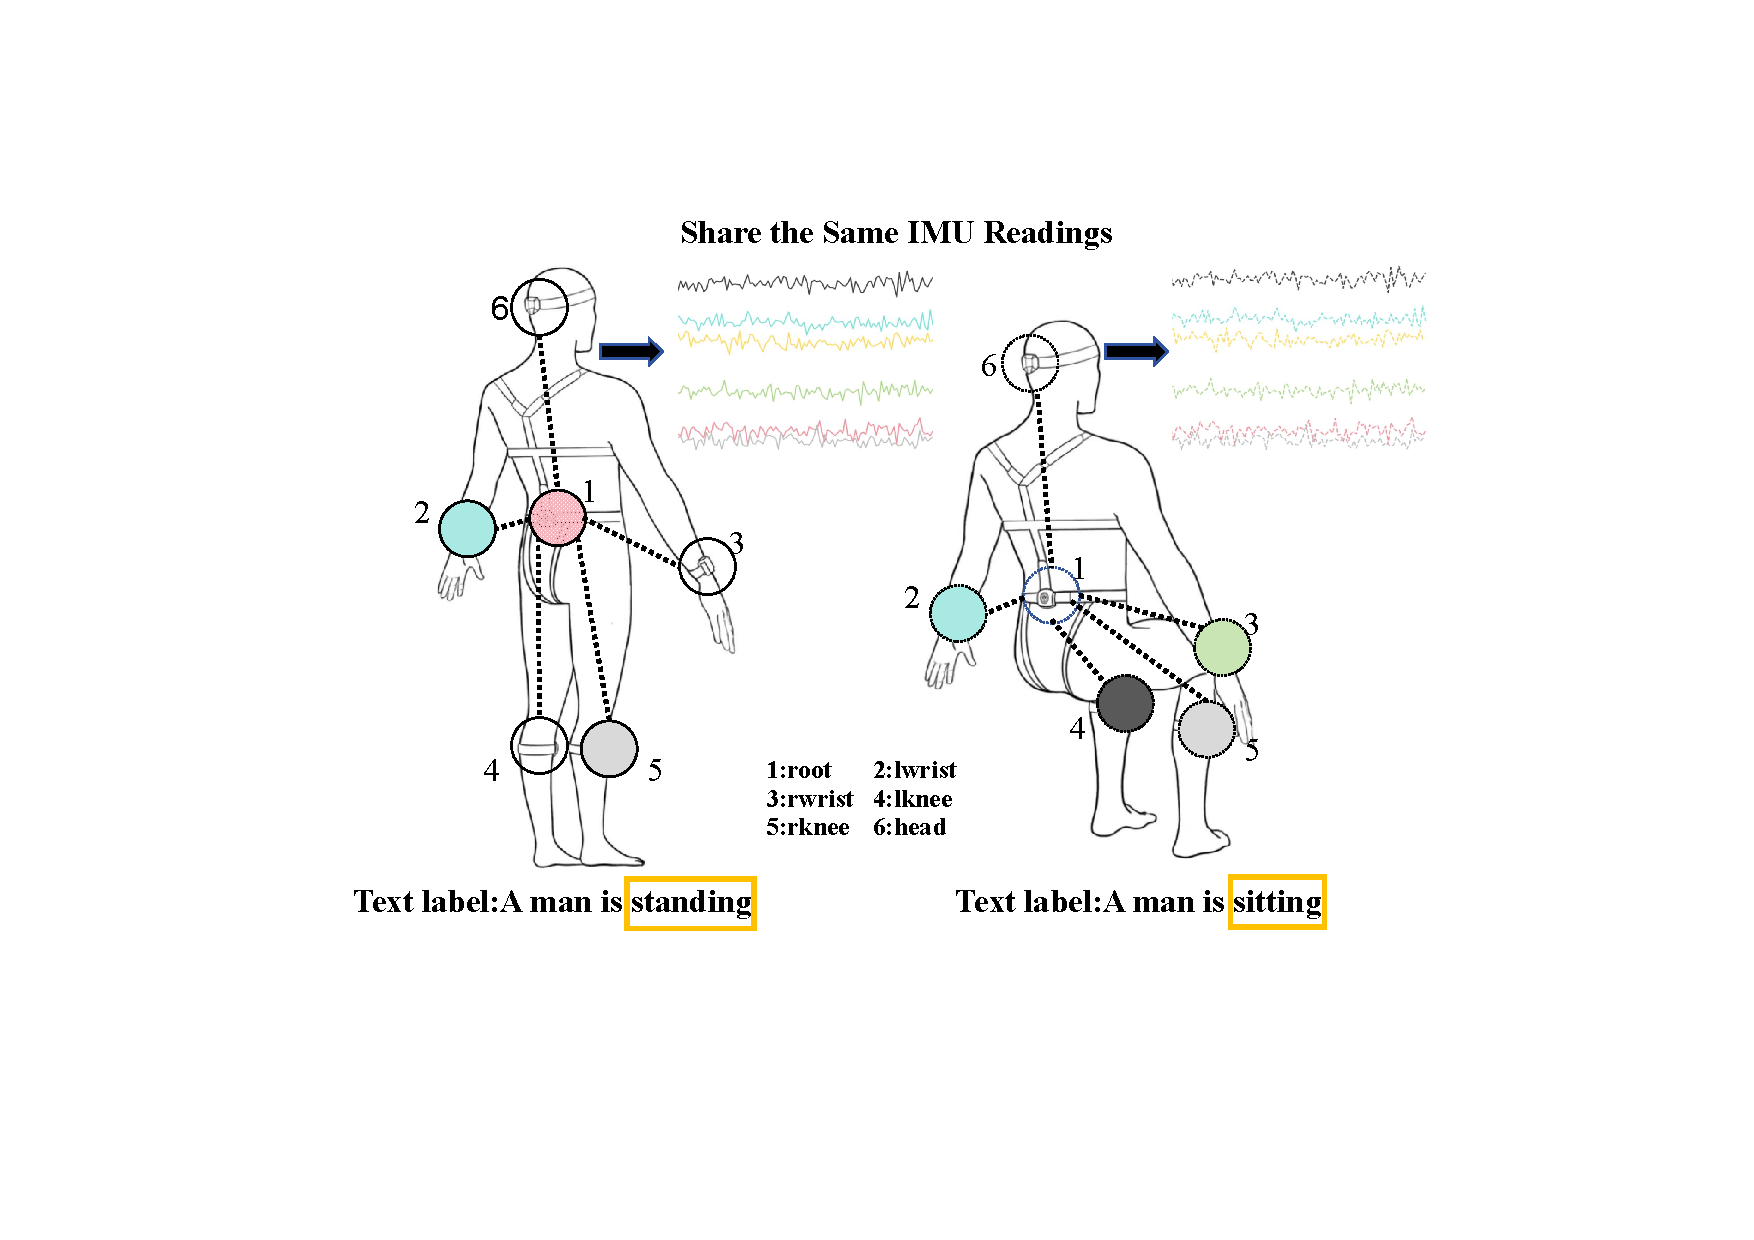
\includegraphics[width=1\columnwidth]{Same_Readings.pdf} 
\caption{Considering specific postures such as standing and sitting, the rotational data and acceleration output by the sensors are largely invariant. Incorporating additional information such as text can help to address this challenge.}
% The sole deviation recorded is the instantaneous acceleration, which occurs during the transition between these states.}
\label{fig1}
\end{figure}
%加上一些简单的文本可以帮助解决
% Concurrently, the swift advancement of wearable devices has given rise to alternative techniques, which capitalize on various sensor devices for human motion reconstruction.

% Relative to optical sensors, IMUs confer several significant advantages including resilience to lighting conditions and occlusions, the freedom of unrestricted movement for both indoor and outdoor activities, and the generation of more naturalistic motion.
% Furthermore, methodologies grounded in inertial sensors can alleviate data privacy issues commonly associated with optical-based solutions.
% In comparison to optical sensors, IMUs provide several notable benefits. These encompass resistance to lighting conditions and occlusions, unrestrained movement for both indoor and outdoor activities, and the generation of more natural motion.
% Moreover, approaches based on inertial sensors alleviate data privacy concerns linked to optical-based solutions.
%不需要对称,inthis paper  tsa  各个模块  contribution


To address this issue, some methods \cite{huang2018deep,yi2021transpose,jiang2022transformer,von2017sparse,yi2022physical} have deployed sparse IMUs on the body and analyzed temporal signals to model human body poses.
These approaches not only reduce the number and cost of IMUs but also enhance the wearability and minimize invasiveness.
% This methodology offers significant advantages in terms of reducing the number and cost of IMUs, as well as providing enhanced ease of
% wearability and reduced invasiveness.
% Nevertheless, dense IMUs placement on the body remains invasive and costly.no
% Nevertheless, certain issues still limit the application of sparse sensors. Specifically, The existing methods face challenges in differentiating between actions that share similar IMUs output patterns. 
Nevertheless, it should be noted that there are still some limitations that restrict the utilization of sparse sensors. 
% existing methods face challenges in differentiating between actions that share similar IMU output patterns.
% as illustrated in Fig. \ref{fig1}, the standing and sitting actions share the same IMU output patterns, which presents a challenge in accurately differentiating between them.
% 
% Specifically, 
% as depicted in Fig. 1, sparse sensors positioned on the body yield similar rotation matrices and acceleration outputs between standing and sitting actions, which is difficult to accurately differentiate them.
Specifically, motion reconstruction using sparse inertial sensors constitutes an under-constrained problem: distinct postures can yield identical sensor outputs. As illustrated in Fig. \ref{fig1}, the sensors generate similar rotation matrices and acceleration outputs when the subject is sitting and standing, making accurate differentiation between these postures challenging.
% as shown in Fig. \ref{fig1}, the standing and the sitting share the same IMU output patterns,  these actions correspond to distinct postures, presenting a challenge in accurately differentiating between them. 
% directly input the output of sparse IMUs for each frame as a token into a temporal analysis network.
% This practice
% Besides, the aforementioned approaches overlooks the inherent distinction of spatial relations (IMU-to-IMU) thereby revealing opportunities for potential enhancements.
% which ignores the natural distinction of spatial relations (IMU-to-IMU), and they are not robust to noise naturally brought by the IMUs, leaving potential improvements on the table.
%太长了
%spatial 先描述下图很少被使用 不用提之前的方法
% Regarding the first issue, several studies have proposed solutions to address the difficulty in distinguishing ambiguous actions. For instance, specialized network design\cite{yi2022physical,jiang2022transformer} or the use of additional sensors\cite{kim2022fusion}.
% \cite{ref3} proposed a learning-based RNN initialization strategy, while  \cite{ref4} Utilized an additional sensor to provide head height information..
% For us, motivated by the recent advancements in natural language processing and multimodal research, We proposed a multimodal fusion framework based on the Transformer architecture which leverages text supervision to accurately model human body poses by incorporating sensor information.
% Besides, the inherent distinction of spatial relations (IMU-to-IMU) shown in the bottom right corner of Fig. \ref{fig1} rarely been used, thereby revealing opportunities for potential enhancements.
Besides, the inherent distinction of spatial relations between IMUs, has rarely been used in previous methods, thereby revealing opportunities for potential enhancements.

% In this paper, inspired by recent advancements in natural language processing and multimodal research, we propose a sensor-based 3D human motion reconstruction with textual supervised framework. 
%明确sensor 我们设计了一个基于对比学习机制  %明确  不能说多模态

% In this paper, we introduce a novel framework for sensor-based 3D human motion reconstruction, leveraging spatial relationships and textual supervision to accurately generate naturalistic human body poses.
In this paper, we introduce a novel framework for sensor-based 3D human motion reconstruction, leveraging spatial relationships and textual supervision to accurately generate naturalistic human body poses.
Sparse sensors are designed to capture the motion characteristics of different body parts. Considering that the correlations among these features contain a crucial priori knowledge about the human body's skeletal structure, our method employs intra-frame spatial attention to model the correlation between IMUs, allowing the model to concentrate on the distinct characteristics of different body regions at one point in time. Moreover, in response to the inherent potential instability of IMU readings, the concept of sensor uncertainty is introduced. This allows for the optimization of sensor outputs and the adaptive adjustment of each sensor's relative contribution. However, relying solely on sensor data is insufficient for resolving the problems of ambiguity. Text, with its rich motion information, can aid the model in identifying human motion states and resolving issues of ambiguity.
% Sparse sensors are designed to capture the motion characteristics of different body parts. Considering that the correlations among these features contain crucial a priori knowledge about the human body's skeletal structure, our method employs intra-frame spatial attention to model the correlation between IMUs. This enables the model to concentrate on the distinct characteristics of different body regions at one point in time. Moreover, in response to the inherent potential instability of IMU signals, the concept of sensor uncertainty is introduced. This innovation allows for the optimization of sensor outputs and the adaptive adjustment of each sensor's relative contribution.
% As illustrated in Fig. 1, six sensors are placed on key locations of the human body, each intended to capture the motion features of the corresponding part. Previous studies often overlook the correlations among these features, yet such relationships contain crucial a priori knowledge about the human body's skeleton structure. In our method, intr-frame spatial attention is employed to model the correlation between different body parts within each frame, thereby enhancing the representation of sensor features. Considering the inherent potential instability of IMU signals, the concept of sensor uncertainty is introduced. This allows for the optimization of sensor outputs and the adaptive adjustment of each sensor's relative contribution.
% The strategic placement of six sensors at pivotal locations along the body's kinetic chain facilitates the acquisition of signals that encapsulate the movement characteristics of the body's primary regions. We contend that the accurate reconstruction of human posture necessitates the modeling of intra-frame spatial correlations which describe the relationships between different body sections.
% As the six sensors are strategically placed along points of the body's kinetic chain, their signals can capture the movement characteristics of different body parts. Therefore, modeling the spatial correlations among sensors within a frame is crucial for accurately modeling human posture. 
% Considering the potential instability inherent in IMU signals, we have introduced the concept of sensor uncertainty. 
% This concept allows for the refinement of sensor outputs and the adaptive adjustment of the relative contributions from each sensor.
% This allows us to refine sensor outputs and appropriately calibrate the relative weights between sensors.
% However, relying solely on sensor data is insufficient for resolving the ambiguities problem. 
% Text, with its rich motion information, can aid the model in identifying human movement states and resolving issues of ambiguity.
% We posit that the rich motion information contained in text can assist the model in accurately discerning human motion states. 
% Moreover, our experimental results have also demonstrated that text contributes to generating more natural and realistic human motions. 
% Finally, to better modality fusion, we propose a unique module designed to align sensor features with text features in both time and meaning.
% Finally, we facilitate modality fusion by achieving temporal and semantic alignment between text and sensor signals.
Finally, to facilitate better modality fusion, we propose unique modules to align sensor features with text features in both temporal and semantic dimensions.

% We posit that text contains rich motion information that can be used to resolve the sitting-standing ambiguity as illustrated in Fig. \ref{fig1}.
% We posit that text provides motion cues that clarify ambiguities such as the sitting-standing distinction shown in Fig. \ref{fig1}. Text labels enable the model to distinguish between these postures accurately. 
% Moreover, our experiment results show that text labels also enhance motion realism, with labels like ``walk like a monkey'' enabling the model to replicate the distinct motion patterns of a monkey's gait.
% We posit that textual information contains rich cues for motion, which can resolve specific ambiguities like the sitting-standing distinction highlighted in Fig. \ref{fig1}. By incorporating textual labels such as ``sitting'' and ``standing'', the model can accurately differentiate between these two postures. Additionally, our experimental evidence suggests that textual information can significantly enhance the generation of natural and coherent movements. For instance, with the inclusion of the label ``walk like a monkey'', the model produces movements that capture the unique dynamics of a monkey's gait. 
% Additionally, the accuracy of motion generation is contingent upon the precise modeling of sensor interconnections. With sensors strategically positioned along the body's kinetic chain, it is imperative to discern the spatial correlations between sensors within a single frame to capture movements accurately. 
% Additionally, with sensors strategically positioned along the body's kinetic chain, it is imperative to discern the spatial correlations between sensors within a single frame to capture specific movements accurately.
% Given the potential instability inherent in IMU signals, we have introduced the concept of sensor uncertainty. This allows us to refine sensor outputs and appropriately calibrate the relative weights between sensors. 
% Finally, we facilitate improved modality fusion by achieving temporal and semantic alignment between text and sensor signals.
% The proposed approach consists of a Sensor-Encoder, 
% a Text-Encoder and a Text-Sensor Fusion Module. 
% In the Sensor-Encoder, the spatial-relation representation is constructed to learn the correlations among the signals from multiple IMUs. Specifically, to tackle the often-overlooked potential instability inherent in IMU signals, an Uncertainty-guided Resampling method is employed, enhancing the robustness of feature extraction. Then, based on the calculated uncertainty of each IMU, we adopt an Uncertainty-guided Spatial Attention (UGSA) mechanism to learn the weighted features of each IMU, corresponding to a specific action at one point in time.
% In the Text-Encoder, the provided text labels are used to extract and emphasize the textual semantics associated with specific actions, such as ``standing'' or ``sitting''.
% Finally, to achieve temporal alignment and fusion between the spatial-relation features from IMUs and the textual semantics, the Text-Sensor Fusion Module is designed to accurately locate and recognize specific actions within the temporal frames.
% In the Text-Sensor Fusion Module, a Hierarchical Temporal Transformer (HTT) based on a local and shifted window attention is utilized. Moreover, we adopt a contrastive learning mechanism to optimize the alignment between the sensor features and textual semantics. 





In the realm of sensor data and text fusion, IMU2CLIP \cite{moon2022imu2clip} bears resemblance to our work, 
aligning images and IMU sensor data with corresponding text using the CLIP \cite{radford2021learning}.
% proposing the alignment of images and IMU sensor readings from smart glasses with their corresponding text within the space of CLIP \cite{radford2021learning}. 
The methodologies diverge in several key respects. IMU2CLIP is designed for modality transitivity, facilitating text-based IMU retrieval, IMU-based video retrieval, and natural language reasoning tasks with motion data. In contrast, our approach underscores the synergistic potential of multimodal information, using text to resolve ambiguities inherent in sparse sensor data. 
Furthermore, to achieve enhanced modality fusion, the Hierarchical Temporal Transformer module was designed, and contrastive learning was employed to ensure temporal and semantic synchronization between the textual and sensor data. Cross-attention mechanisms were then utilized to merge features from both modalities.
% Furthermore, a model has been developed that captures the spatial correlations among six sensors strategically positioned across the body, significantly enhancing sensor feature representation. 
% Lastly, IMU2Clip utilizes image data from smart glasses, together with corresponding sensor data and text, which are different from ours.
% However, their approach primarily targets modality transitivity, enabling text-based IMU retrieval, IMU-based video retrieval, and natural language reasoning with motion data, rather than capturing subtle bodily motions. In contrast, our methodology enhances the detection of fine motor movements through spatial correlation modeling across six body-mounted sensors, enriched by textual data. We prioritize the synergistic use of multimodal information to resolve the ambiguities inherent to motion capture with sparse inertial sensors, thus producing precise and lifelike human motion.
 % In the realm of sensor data and text fusion, IMU2CLIP \cite{moon2022imu2clip}  bears resemblance to our work, proposing the alignment of images and IMU sensor readings from smart glasses, and their corresponding text within the high-dimensional space of CLIP \cite{radford2021learning}. However, their approach is designed to focus on transitivity between modalities, facilitating text-based IMU retrieval, IMU-based video retrieval, and natural language reasoning tasks with motion data, rather than the discernment of nuanced bodily motions.
 % Our methodology, in contrast, refines the detection of fine motor movements through spatial correlation modeling across six body-mounted sensors, supplemented by text. We focus on the synergistic use of multimodal information to eliminate the ambiguities of motion capture using sparse inertial sensors, thereby generating precise and natural human motion.
% In the realm of sensor data and text fusion, IMU2CLIP \cite{moon2022imu2clip} shares similarities with our work, which proposed a novel pre-training strategy to align IMU recordings with corresponding videos and textual data within the joint representation space of CLIP \cite{radford2021learning}.
% Our work is most closely related to IMU2CLIP \cite{moon2022imu2clip}, which proposed a novel pre-training strategy to align IMU recordings with corresponding videos and textual data within the joint representation space of CLIP \cite{radford2021learning}. However, their approach is designed to focus on transitivity between modalities, facilitating text-based IMU retrieval, IMU-based video retrieval, and natural language reasoning tasks with motion data. In contrast, our method specifically focuses on the synergistic use of multimodal information to model human poses with high precision.
Experimental results show that our proposed framework achieves state-of-the-art performance compared with some classical methods, both in quantitative and qualitative measurements.
% Particularly, sensor sequences and corresponding text labels are separately fed into individual encoders for feature encoding. For the sensor encoder, spatial and temporal modeling of sensor data has been carried out to better represent the complex relationships inherent in the sensor readings.
 % In the realm of spatial modeling,
% considering the instability of the spatial relationships reflected by the sensors, we propose a Unertainty-guided Spatial Attention Module for modeling intra-frame IMU relations while considering the prediction uncertainty. In terms of temporal modeling, a Hierarchical Temporal Transformer is introduced. By employing local window attention, shift window attention, and a patch merging strategy, this aspect of the model seeks to mitigate the computational load typically associated with global attention.
% The text encoder is employed to capture the textual features within the text labels that are most highly correlated with motion information, such as standing.
% Subsequently, we design a mechanisms based on contrastive learning to align the two features originating from sensor and text, and cross-attention is utilized for feature fusion, culminating in the generation of refined human poses.
% We employ contrastive learning to align the two features derived from different modalities and utilize cross-attention mechanisms to fuse multi-modal features.
% thereby accurately modeling human posture.

% We have conducted spatial and temporal modeling of motion features.
% In the realm of spatial modeling, considering the instability of the spatial relationships reflected by the sensors, we propose a Unertainty-guided Spatial Attention Module for modeling intra-frame IMU relations by explicitly considering the prediction uncertainty. The Uncertainty-guided Spatial Attention Module includes a sampling strategy and a spatial-Attention mechanism, both guided by estimated uncertainty for each IMU. New IMUs readings are sampled using a Gaussian distribution with uncertainty as variance, enhancing error-resilience. High-uncertainty IMUs are then minimized in learning through the Uncertainty-Guided Spatial-Attention, improving the model's robustness. 
% This method involves regression to obtain the certainty of each sensor and diminishes the contributions of sensors with low certainty.
%写一下具体的怎么做明确输入 具体谈一下怎么做(文本) 空间对于传感器而言,考虑到传感器反应的空间关系具有不确定性,我们提出一个基于传感器确定性计算的相对  模型 怎么融合 
%引入文本 对比学习
%确定性引导
% In the realm of spatial relationship modeling, we have not merely employed standard techniques such as graph convolution\cite{kipf2016semi} or transformer\cite{vaswani2017attention} modules. Instead, we introduce an Uncertainty-guided Refinement Network (UGRN) along with an Uncertainty-guided Spatial Transformer(UGST). The primary aim of these methods is to refine the readings from IMU, as well as to delve into the spatial relationships amongst various IMUs. This refined model assimilates the estimated uncertainty of each IMU, which represents confidence level of the current sensor data with respect to posture. Subsequently, new IMU readings are drawn from a Gaussian distribution centered around the original readings, wherein the uncertainty serves as the variance and prior readings act as the mean. Finally, the UGST employs a Uncertainty-guided self attention mechanism to model spatial relationships among IMUs while concurrently diminishing the impact of high uncertainty. 
% With respect to temporal modeling, to alleviate the computational burden associated with global attention, we introduce a Hierarchical Temporal Transformer (HTT), inspired by the principles of the Swin \cite{liu2021swin}. The HTT computes its representation using local windows, shift windows, and a patch merging strategy.
% In terms of temporal modeling, a Hierarchical Temporal Transformer is introduced. By employing local window attention, shift window attention, and a patch merging strategy, this aspect of the model seeks to mitigate the computational load typically associated with global attention.
% With respect to temporal modeling, we introduce a Hierarchical Temporal Transformer. By utilizing local window attention, shift window attention, and a patch merging strategy to model time information, we aim to alleviate the computational burden associated with global attention.
In summary, our work makes the following contributions:
\begin{itemize}
\item We present a sensor-based approach to 3D human motion reconstruction that is augmented with textual supervision. This method leverages the rich semantic information contained within the text to enhance the naturalness and precision of the modeled human poses.
\item 
We introduce a spatial-relation representation model which computes the correlations between sensors within a frame while also taking into account the uncertainty of each IMU.
% We present a spatial-relation representation model based on IMUs' signals. Specifically, it constructs the spatial relations between the signals, taking into account the uncertainty of each IMU.
% and augment the system's robustness against ambiguous action.
\item 
We design a Hierarchical Temporal Transformer module to achieve temporal alignment between sensor features and textual semantics. A contrastive learning mechanism is also adopted to optimize the alignment between the two modalities in high-dimensional space.
\end{itemize}

% In addressing the challenge of distinguishing ambiguous actions, our approach takes inspiration from recent advancements in natural language processing and multimodal research. We propose a multimodal fusion framework based on the Transformer architecture, leveraging text supervision to accurately model human body poses by integrating sensor information. 
% In response to the first issue, numerous studies have proposed solutions to tackle the challenge of distinguishing ambiguous actions. These include specialized network designs \cite{yi2022physical,jiang2022transformer} and the utilization of additional sensors \cite{kim2022fusion}.
% Our approach, inspired by recent advancements in natural language processing and multimodal research, proposes a multimodal fusion framework. This is based on the Transformer architecture and leverages text supervision to model human body poses accurately by integrating sensor information.
% We posit that enriching the motion data with semantic information can facilitate the reconstruction of more precise and less ambiguous body poses.

% For the second problem,we present an UGST(Uncertainty-guided Spatial Transformer) to refine imu reading, by considering the estimated uncertainty of each imu with Uncertainty-guided sampling strategy and self-attention mechanism.The uncertaintyguided sampling strategy incorporates the estimated uncertainty for each imu (that implies the noise of imu reading) into the learning procedure. The new imu readings are sampled around the original imu readings following a Gaussian distribution with the estimated uncertainty as variance. Then, we use the sampled readings as the input of UGST to make the model more robust to noise. The UGST is developed to reduce the contribution of the imus with high uncertainty during learning.
% To tackle the second challenge, we introduce an Uncertainty-guided Refinement Network (UGRN) along with an Uncertainty-guided Spatial Transformer(UGST). The primary aim of these methods is to refine the readings from IMU, as well as to delve into the spatial relationships amongst various IMUs. 
% This advanced model incorporates each IMU's estimated uncertainty, representing noise. And then new IMU readings are sampled around original readings via a Gaussian distribution, with the uncertainty as variance and old readings as mean, thereby enhancing noise robustness.
% This refined model assimilates the estimated uncertainty of each IMU, which signifies noise. Subsequently, new IMU readings are drawn from a Gaussian distribution centered around the original readings, wherein the uncertainty serves as the variance and prior readings act as the mean. This approach effectively bolsters the model's resilience to noise. 
% Finally, the UGST employs a Uncertainty-guided self-attention mechanism to model spatial relationships among IMUs while concurrently diminishing the impact of high uncertainty. 


% However, the sparse sensor information introduces ambiguity during the modeling process, making it challenging to distinguish between certain actions.For instance, considering the actions of standing and sitting, the output of inertial sensors remains largely invariant. Nevertheless, these actions correspond to distinct postures, presenting a challenge in accurately differentiating between them. \cite{ref3} proposed a learning-based RNN initialization strategy, while  \cite{ref4} utilized past pose outputs as inputs.

% Motivated by the recent advancements in natural language processing and multimodal research, we present an attention-based multimodal model that leverages text supervision to accurately model human body poses by incorporating sensor information.

% Our algorithm has three stages: 1)We first encode the motion and text independently with a motion encoder and a text encoder.2)Then, Aligning motion features and text features in the clip feature space using contrastive learning.3)Next, we employ a multimodal encoder to merge the image features with the text features using crossmodal attention.



% To validate the effectiveness of our approach, we evaluate it on publicly available datasets and compare it with previous methods. Our method outperforms the state-of-the-art techniques across multiple metrics, showcasing its efficacy.



% \begin{figure}[t]
% \centering
% \includegraphics[width=0.9\columnwidth]{CameraReady/LaTeX/Figure31.png} 
% % Reduce the figure size so that it is slightly narrower than the column. Don't use precise values for figure width.This setup will avoid overfull boxes.
% \caption{our model encapsulates three distinct encoders: a text encoder, a motion encoder, and a multimodal encoder.
% We utilize contrastive learning to align the unimodal representations of motion-text pairs prior to multimodal fusion.
% }
% \label{fig2}
% \end{figure}
% , uncertainty estimation, and spatial attention mechanisms 
\section{Related Work}
% In the field of motion reconstruction, significant research has focused on capturing human motion using a range of inputs, primarily through methods based on visual and inertial sensor data. Our review primarily focuses on previous works that hold the greatest relevance to our study, specifically those that rely on inertial sensors (or in combination with other information) for motion reconstruction. Moreover, we introduce some studies pertinent to the application of textual semantic information in the field of human motion, which have provided partial inspiration for our research.
% In the field of motion reconstruction, significant research has focused on capturing human motion using a range of inputs, with an emphasis on methods based on visual and inertial sensor data. Our review concentrates on the most relevant previous works to our study, specifically those utilizing inertial sensors, either exclusively or in conjunction with other data, for motion reconstruction. Additionally, we discuss studies that apply textual semantic information to human motion, which have also partially inspired our research.

% We mainly reviewed previous works that are most relevant to our work, specifically those based on inertial sensors(or combineed with other information) for motion reconstruction. In addition, we also introduced some works related to the application of multimodal fusion , uncertainty estimation and spatial attention mechanisms in the field of human motion. 
% specifically those based on the Transformer architecture. The Transformer constitutes the core of our reconstruction model, and 
% These works have partially inspired our research.
\begin{figure*}[!t]
\renewcommand{\baselinestretch}{1.0}
\centering 
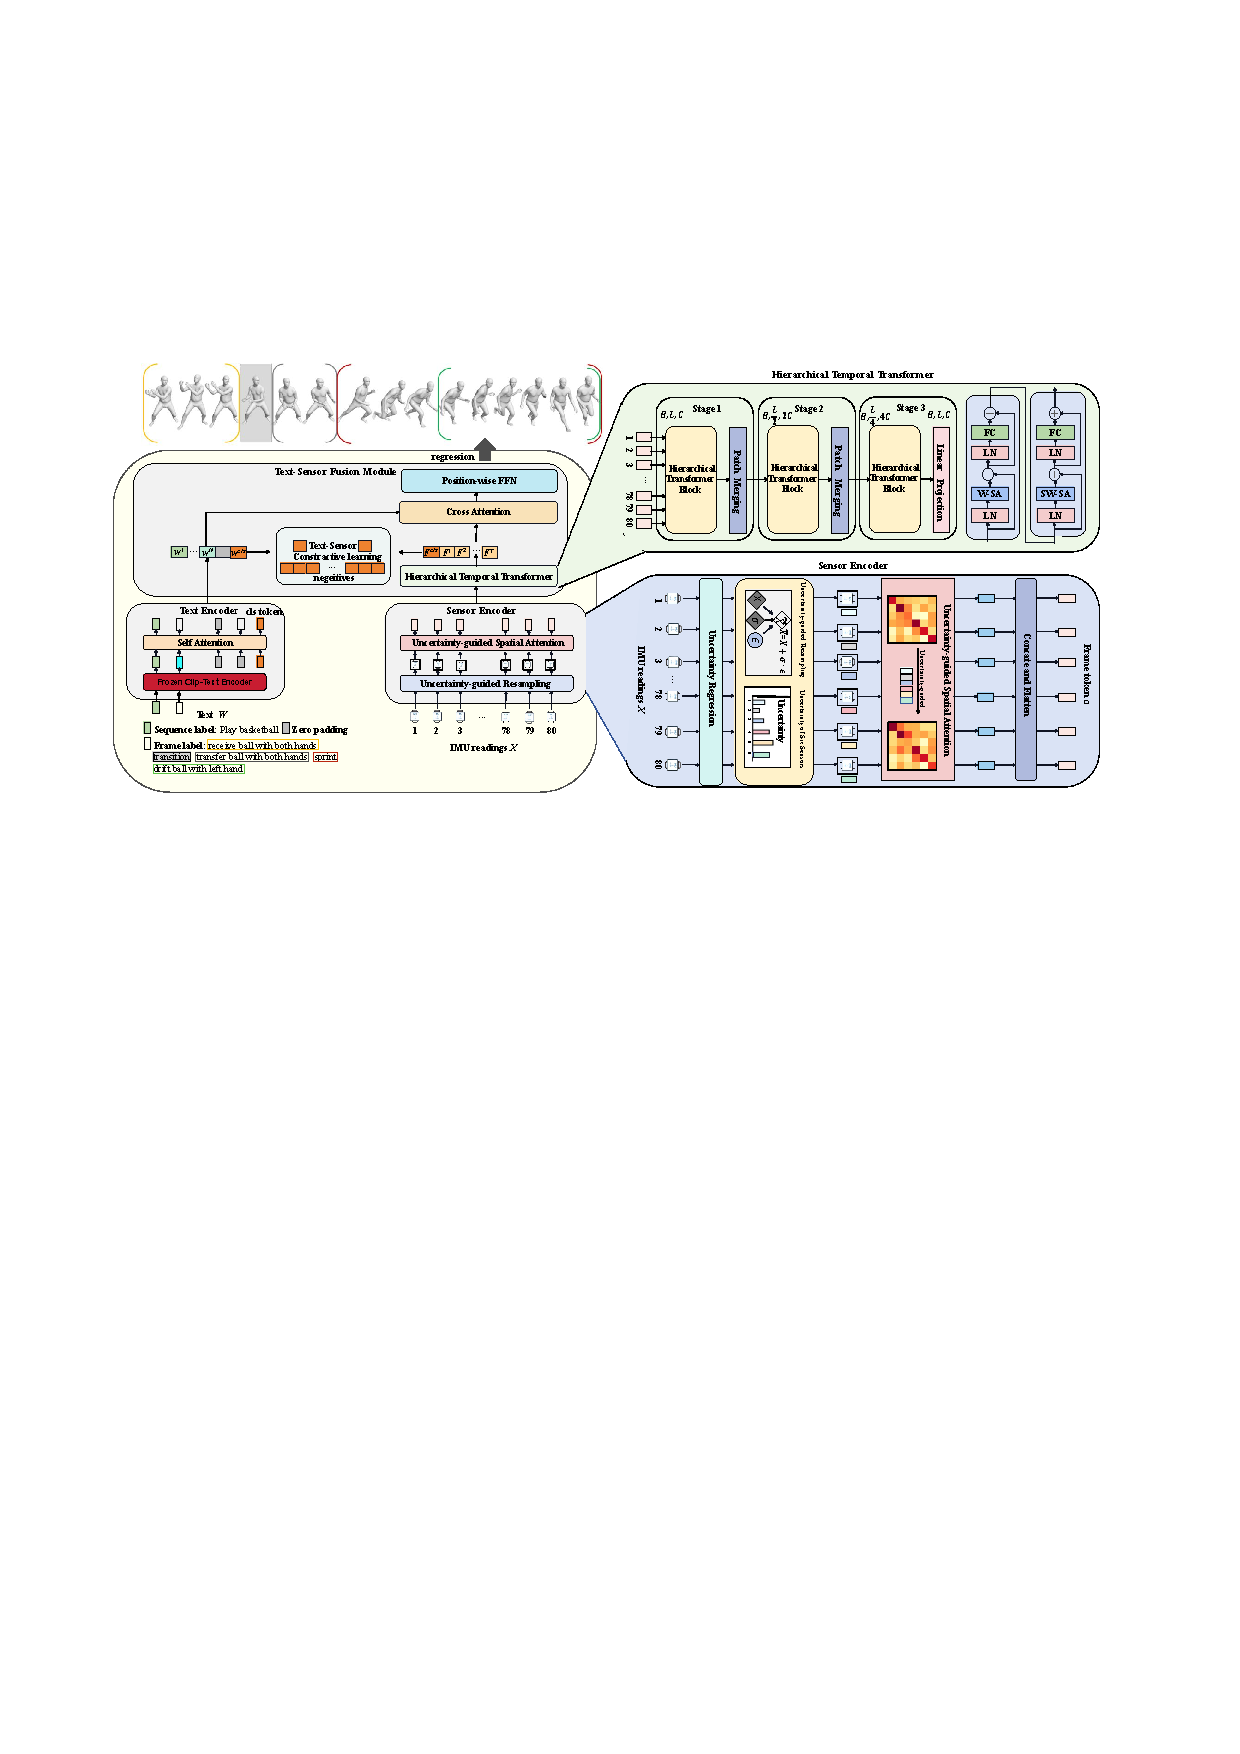
\includegraphics[width=7 in, height=3 in]{net_result.pdf}
\caption{Overview of our method. Our model encapsulates three distinct encoders: a Text Encoder, a Sensor Encoder, and a Text-Sensor Fusion Module. The details of the Sensor Encoder and the Hierarchical Temporal Transformer module are illustrated on the right. The schematic of the model output is adapted from \cite{BABEL:CVPR:2021}.}\label{fig2}
\end{figure*}
\subsection{Sensor-based Human Motion Reconstruction}
Full-body sensor-based motion reconstruction is a widely utilized technique in commercial motion capture systems. A prominent example is the Xsens system \cite{schepers2018xsens}, which achieves detailed reconstruction of human movements by equipping the body with 17 strategically placed IMUs.
However, this method presents drawbacks, primarily its invasive impact on human movement due to the intensive IMUs placement, as well as its substantial cost.

Efforts have been made to implement motion reconstruction using sparse IMUs, thereby enhancing the usability of inertial sensor-based motion reconstruction, albeit at the expense of some degree of accuracy. For instance, studies \cite{slyper2008action,tautges2011motion} have achieved human motion reconstruction with as few as four to five accelerometers, by retrieving pre-recorded postures with analogous accelerations from motion reconstruction databases. \cite{von2017sparse} developed an offline system that operates with only six IMUs, optimizing the parameters of the SMPL body model \cite{loper2015smpl} to fit sparse sensor inputs. With the advent of the deep learning era, \cite{huang2018deep} synthesized inertial data from an extensive human motion dataset to train a deep neural network model based on a Bidirectional Recurrent Neural Network that directly mapped IMU inputs to body postures. \cite{yi2021transpose} decomposed body posture estimation into a multi-stage task to improve the accuracy of posture regression through the use of joint locations as an intermediate representation. Moreover, recent methodologies such as \cite{dittadi2021full} and AvatarPoser \cite{jiang2022avatarposer} estimated full-body posture using only head and hand sensors, yielding promising results.

However, reconstructing human motion from a set of sparse IMUs presents an under-constrained problem, where similar sensor readings may correspond to different postures. Some approaches have sought to address this issue to a certain extent through unique network designs. For instance, Physical Inertial Poser \cite{yi2022physical} approximated the under-constrained problem as a binary classification task between standing and sitting, proposing a novel RNN initialization strategy to replace zero initialization. It then distinguished between standing and sitting based on instantaneous acceleration. Transformer Inertial Poser \cite{jiang2022transformer} introduced past history outputs as inputs to differentiate ambiguous actions. 
Other methodologies have explored the integration of multimodal information to impose additional constraints on the model, enhancing the generation of precise poses. For instance, studies \cite{von2018recovering,malleson2017real,von2016human} have significantly improved estimation accuracy by combining inertial sensors with video data, although challenges such as occlusion, lighting issues, and mobility restrictions still persist. Fusion Poser \cite{kim2022fusion} incorporates head height information from a head tracker into the model's input.


% For instance, PIP \cite{yi2022physical} reframes the under-constrained problem as a binary classification task between standing and sitting. It proposes a novel RNN initialization strategy to replace zero initialization and discriminates between standing and sitting based on instantaneous acceleration. TIP \cite{jiang2022transformer} incorporates past output history as input to differentiate ambiguous actions.
% Other methodologies aim to integrate multimodal information to impose additional constraints on the model for accurate posture generation. For example, studies \cite{von2018recovering,malleson2017rea,von2016human} have significantly improved estimation accuracy by combining inertial sensor data with video data, despite persistent challenges such as occlusion, lighting issues, privacy concerns, and mobility restrictions. Fusion Poser \cite{kim2022fusion} partially addresses the problem by combining IMU data with the head height information returned from a head tracker.
\subsection{Textual Semantics in Human Motion Field}
In the burgeoning field of multimodal processing, text, with its rich semantic information and ease of annotation, is increasingly utilized in the human motion domain. Studies such as \cite{guo2022generating,zhang2022motiondiffuse,tevet2022motionclip} can generate high-quality 3D human motions from textual descriptions. 
These findings affirm that texts encapsulate rich motion information. We posit that text supervision could disambiguate actions, thereby enhancing the naturalness and precision of generated motions.

% In our task, we face the additional challenges of accurately modeling sensor data and mitigating noise from real IMU sensors. Notably, while previous methods focus on the temporal modeling of sensor data, spatial modeling between frames is often overlooked. In the realm of human motion, spatial attention is widely employed. For instance, \cite{aksan2021spatio} devised a generative model with a dual-attention mechanism to reconstruction spatial and temporal correlations, enabling the prediction of imminent full-body motions. \cite{zheng20213d} designed a spatial-temporal transformer that meticulously models the relationships of human joints within and across frames to yield an accurate 3D human pose. This spatial attention mechanism was further utilized in subsequent work \cite{zhao2023poseformerv2}. We leverage spatial attention in our task to model the relationships between each frame of IMU data.

% In our task, we face additional challenges of accurately modeling sensor information and handling noise from real IMU sensors. Specifically, previous methods have emphasized temporal modeling of sensor information, neglecting spatial modeling between frames. In the human motion field, spatial attention has been widely adopted. \cite{aksan2021spatio} developed a generative model that leverages a dual-attention mechanism to reconstruction spatial and temporal correlations, enabling the prediction of full-body motions in the near future within a short time frame. \cite{zheng20213d} designed a spatial-temporal transformer structure that meticulously models the relationships of human joints within each frame and the temporal correlations across frames in order to output an accurate 3D human pose of the center frame. This spatial attention mechanism was further utilized in the subsequent work\cite{zhao2023poseformerv2}. We apply spatial attention to our task, modeling the relationships between each frame of IMUs data.

% Regarding noise handling, previous methods have noted that synthetic IMU data and real IMU data exhibit distinct noise distributions. \cite{yi2021transpose} suggests training models solely on synthetic data first, then fine-tuning them on a smaller real dataset. \cite{jiang2022transformer} proposes a simple sliding average filter to align the distribution of synthetic and real data, but neither explicitly model noise. In our work, we aim to explicitly model noise through uncertainty. Several methodologies have introduced the concept of uncertainty into the domain of motion analysis. \cite{song2021uncertain} contemplated the uncertainty inherent in noisy input data and proposed the Uncertain Graph Neural Networks for the detection of facial action units. Concurrently, \cite{li2023pose} introduced an Uncertainty-guided refinement network aimed at enhancing pose predictions for challenging joints. 
% % This was achieved through an Uncertainty-guided sampling strategy and the implementation of a self-attention mechanism. 
% In our work, we employ uncertainty analysis on sensor input data, enhancing the model's robustness to noise.
%这里得引入文本信息了
\section{Method}
%逻辑混乱 先讲文本的,再讲运动的
% Our goal is to obtain an accurate human pose from 6 IMUs placed on the user’s legs, wrists, head, and pelvis, and the corresponding semantic information.In adherence to previous research methodologies, we employ the tri-axial acceleration and rotation matrix data outputs derived from each frame of the six sensors as model input.
Our primary target is to reconstruct accurate human poses using data from 6 IMUs placed on the legs, wrists, head, and pelvis (root), coupled with textual supervision. The sensors provide inputs in the form of tri-axial acceleration, $a \in \mathbb{R}^{3}$, and rotation matrices, $R \in \mathbb{R}^{3\times3}$.
%sensor text输入
% To create the text encoder, We have incorporated the first four frozen layers from the CLIP's ViT/B32 model, supplemented by an additional two Transformer layers. 
% The UGRT and UGST are employed to reconstruction spatial correlations among the six sensors and augment the system's robustness, while the Hierarchical Temporal Transformer is utilized to extract temporal dependencies within the motion sequence efficiently.
%解释
% where mcls represents the embedding of the [CLS] token. 
% In the realm of modality fusion, we employ a four-layer transformer predicated upon local window attention as the underpinning for our multimodal encoder. 
% which is not detailed in Figure \ref{fig2}.明确输出 提对比学习
As illustrated in Fig. \ref{fig2}, our framework consists of a Text Encoder, a Sensor Encoder, and a Text-Sensor Fusion module. 
The Text Encoder converts the input text $W$ such as [“receive ball with both hands”, ..., “transition”] into a sequence of embeddings: $\{W^{cls}, W^{1}, ..., W^{N}\}$, where $W^{cls}$ represents the embedding of the [CLS] token, and $N$ denotes the number of text labels. 
For the Sensor Encoder, 
a motion sequence composed of sensor data frames 
$X^{t}=[(a_{root}^t,R_{root}^t),..., (a_{head}^t,R_{head}^t)], t \in [1,T]$ 
is encoded into a sequence of embeddings that contain intra-frame spatial relations: $\{O^{1}, ..., O^{T} \}$. 
% (a_{root}^t,R_{root}^t),...,(a_{head}^t,R_{head}^t) , t \in [1,T]
Within the Text-Sensor Fusion module, these spatial embeddings are then processed by the Hierarchical Temporal Transformer to extract a unified spatio-temporal fusion representation $\{{F^{cls}, F^{1}, ..., F^{T}}\}$, where $F^{cls}$ denotes the embedding of the [CLS] token.
Before applying cross-attention in the fusion process, Text-Sensor contrastive learning is strategically implemented to refine the alignment between the unimodal representations of the two modalities.
Finally, a simple regression head is employed to derive human pose rotational data $q \in \mathbb{R}^{j\times6}$ for $j$ key points (with each rotation encoded by a 6D vector \cite{zhou2019continuity}), the corresponding three-dimensional position $p \in \mathbb{R}^{j\times3}$, and the root's speed data $s \in \mathbb{R}^{3}$.
%这里得改
% We employ contrastive learning to align the features from both sensors and text within a high-dimensional space. These features are then harmoniously fused through cross attention within the Text-Sensor Fusion Module. Subsequently,

\subsection{Text Encoder} 
% We employ the first 4 layers of the frozen CLIP VIT/B32 text encoder in conjunction with two transformer layers. 
% 改 中式英文
% This forms our text encoder, transforming the input text and an additional [CLS] token into a sequence of text embeddings $\{wcls, w^{1}, ..., w^{N}\}$. The $wcls$ token is used to summarize the input text.
We utilize the first 4 layers of the frozen CLIP \cite{radford2021learning} VIT/B32 text encoder, augmented with two additional transformer layers, to form our Text Encoder. Specifically, given a text label sequence $W$, it is initially tokenized and mapped into a sequence of tokens $\widetilde{W}$ using CLIP, with a zero-initialized tensor prepended as the [CLS] token. It is important to note that $W$ provides two kinds of semantic labels: sequence-level and frame-level labels, as defined in the dataset configuration. For frame-level labels, despite each frame having its own text description, they are largely repetitive. For example, the label ``walk'' might apply continuously over a series of frames. To mitigate computational load, only non-repetitive frame-level texts are chronologically ordered as inputs. For sequence labels, if the total number is less than the threshold $M$, we use all sequence labels as input. Otherwise, one-third of the labels are selected based on their temporal information, specifically choosing those that best match the sensor subsequence.
% we select sequence labels equivalent to one-third of the total sequence number that best match the motion subsequence by using temporal information. 
% To differentiate sequence-level and frame-level labels, two learnable group encodings $G$ for each are developed. Additionally, Sinusoidal Position Encoding\cite{vaswani2017attention} $T$ are utilized based on their temporal information. 
To differentiate between sequence-level and frame-level labels, two learnable group position embeddings \(G\) are developed for each. Additionally, Sinusoidal Position Embeddings \cite{vaswani2017attention} 
\(P\) are utilized, with time information computed independently for both the sequence and frame levels, accommodating their unique characteristics.
\begin{equation}
     \overline{W}^{i} = \widetilde{W}^i+P^i +G^{i}, ~~ for~~ i\in [1,N]
\end{equation}
Then the processed features $\overline{W}$ and the [CLS] token are fed into the self-attention layers to better extract textual semantics.
%最后学出了什么textual semantic
\subsection{Sensor Encoder} 
% The sensor encoder captures the intricate relationships within sensor data through spatial modeling, utilizing an Uncertainty-guided Spatial Attention Module and a Hierarchical Temporal Transformer. The former reconstructs inherent spatial sensor relationships, considering the uncertainty of the IMUs, while the latter deciphers the temporal relationships in motion sequences. The harmonization of spatial and temporal data representations through these modules contributes to the enhancement of the overall model's performance.
% The sensor encoder is designed to capture the intricate relationships within sensor data through both spatial and temporal modeling, which include a Uncertainty-guided Spatial Attention Module with a Hierarchical Temporal Transformer. The former module is designed to reconstruct inherent spatial sensor relationships, taking into account the associated uncertainty of the IMUs. In contrast, the latter module is focused on deciphering the temporal relationships inherent in motion sequences. The harmonization of spatial and temporal data representations through these modules contributes to the enhancement of the overall model's performance.
% The first module reconstruct inherent spatial sensor relationships while considering the uncertainty of IMUs. The latter module detects temporal relationships within motion sequences, harmonizing spatial and temporal data representation for improved model performance.
% The Motion Encoder
% % , with its three distinct networks, optimizes IMU data utilization for feature extraction. These networks 

% Motion Encoder aims at better utilizing the imu information for feature extracting.It encompasses three distinct networks: the Uncertainty-guided Refinement Network, the Uncertainty-guided Spatial Transformer, and the Hierarchical Temporal Transformer, as shown in Fig\ref{fig:3} The initial two modules in our system are designed to apprehend the inherent spatial relationships between sensors while augmenting the model's robustness against noise. On the other hand, the final module is dedicated to capturing temporal relationships within the motion sequences. This comprehensive approach ensures a meticulous interpretation of the data, integrating both spatial and temporal dimensions, ultimately enhancing the model's accuracy and performance.
The Sensor Encoder captures the intricate relations within sparse sensors via spatial modeling. It includes a resampling strategy and a spatial attention mechanism, both guided by estimated uncertainty for each IMU.   

\textbf{Uncertainty Estimation:}
First, we estimate the uncertainty for each IMU reading, where the original IMU readings, denoted by $X^{t} \in \mathbb{R}^{6\times(3+3\times3)}$ are fed into an uncertainty regression head, yielding uncertainty $\sigma^{t} \in \mathbb{R}^{72}$ for each channel.
% We first model the uncertainty for each imu reading. Specifically, original imu readings $\bar{Y} \in R^{72}$ are sent to an uncertainty estimation head, producing the uncertainty $\sigma \in R^{72}$ for each channel of the IMU.
% In lieu of directly applying the initial original imu readings$\bar{Y}$, our approach involves the random sampling of imu readings $\widetilde{Y}$ around original imu readings$\bar{Y}$. This sampling follows a Gaussian distribution $\mathcal{N}(\mu, \sigma^2)$, where the predicted uncertainty $\sigma$ serves as the variance and $\bar{Y}$ serve as mean. $\widetilde{Y}$ are then inputted into the UGST. 
% Rather than leveraging the original initial IMU readings, denoted as $\bar{Y}$, our methodology involves the stochastic sampling of IMU readings, symbolized as $\widetilde{Y}$, around the initial readings $\bar{Y}$. This sampling procedure adheres to a Gaussian distribution $\mathcal{N}(\mu, \sigma^2)$, wherein the predicted uncertainty $\sigma$, acts as the variance and $\bar{Y}$ assumes the role of the mean. Subsequently, these sampled readings, $\widetilde{Y}$, are fed into the UGST.
% It's noteworthy that this sampling technique is exclusively employed during the training phase. During the inference stage, we merely regress the uncertainty across each sensor channel and input the original sensor readings as $\widetilde{Y}$ into the UGST. 
% To facilitate accurate back-propagation, we utilize a reparameterization trick\cite{kingma2013auto}, which allows us to randomly draw a sample from the standard Gaussian distribution $\mathcal{N}(0, 1)$, $i.e.$, $\epsilon \sim\mathcal{N}(\textbf{0},\textbf{1})$.
% Then the sampled readings $\widetilde{Y}$ are then fed into the UGST.

\textbf{Uncertainty-guided Resampling:}
Rather than directly using the original readings $X^{t}$, we resample IMU readings denoted as $\widetilde{X}^{t}$ from a Gaussian distribution $\mathcal{N}(X^{t}, \sigma^{t})$, with $X^{t}$ as the mean and predicted uncertainty $\sigma^{t}$ as the variance. This resampling method ensures that the values with low uncertainty remain largely unchanged, while the values with high uncertainty are resampled, thereby optimizing the sensor data.
Notably, the resampling procedure is only employed during the training. During inference, the uncertainty is simply regressed for each channel, and the original sensor readings $X^{t}$ are utilized as $\widetilde{X}^{t}$.
% The sampling procedure is exclusively employed during the training phase, and during inference, we only regress the uncertainty for each sensor channel and use the original sensor readings as $\widetilde{Y}$.
We apply the reparameterization trick \cite{kingma2022autoencoding} for efficient gradient descent by sampling $\epsilon \sim\mathcal{N}(\textbf{0},\textbf{1})$ to compute $\widetilde{X}^{t}$ as follows: $\widetilde{X}^{t} =X^{t}+\sigma^{t} \cdot \epsilon$ .


\textbf{Uncertainty-guided Spatial Attention (UGSA):}
% Upon acquisition of the i-th frame's sampled IMU readings, denoted as $\widetilde{Y}^{i}$, and their corresponding uncertainties$\sigma^{i}$. We project $\widetilde{Y}^{i}$ into feature embeddings, denoted as ${Z}^{i} \in R^{6\times C}$,where C is the spatial embedding dimension, and equip ${Z}^{i}$ with positional embeddings. Subsequently, these results are forwarded to the Transformer layer within the UGST. 
% We then enrich ${Z}^{i}$ with positional embeddings, and these augmented representations are subsequently forwarded to the Transformer layer embedded within the UGST.
% The layer bears resemblance to the standard Transformer\cite{vaswani2017attention},
% Upon obtaining the sampled IMU readings for the $t$-th frame, represented as $\widetilde{X}^{t}$, along with their corresponding uncertainties $\sigma^{t}$, we project $\widetilde{X}^{t}$ into a feature embeddings space, symbolized as ${Z}^{t} \in \mathbb{R}^{6\times c}$. Here, 6 corresponds to the six sensors, and $c$ signifies the spatial embedding dimension. We then conduct self attention \cite{vaswani2017attention} on ${Z}^{t}$.
% It is noted that for the computation of $t$-th frame's attention between two sensors, denoted as $j$ and $k$, the uncertainty $\sigma_{k}^{t}\in \mathbb{R}^{12}$ (summed over its 12 channels) is taken into account by dividing the attention score by it. 
After sampling the IMU readings for the \(t\)-th frame \(\widetilde{X}^{t}\) with corresponding uncertainty \(\sigma^{t}\), we map \(\widetilde{X}^{t}\) to a \(6 \times c\) feature embedding \(Z^{t}\), where 6 represents the number of sensors and \(c\) signifies the dimension of spatial features. We then conduct self-attention \cite{vaswani2017attention} on ${Z}^{t}$.
It is noted that for the computation of $t$-th frame's attention between two sensors, denoted as $j$ and $k$, the uncertainty $\sigma_{k}^{t}\in \mathbb{R}^{12}$ (summed over its 12 channels) of sensor $k$ is taken into account by dividing the attention score by it. 
\begin{equation}
A_{j,k}^{t}=\frac{\left(Z_j^{t} P^Q\right)\left(Z_k^{t} P^K\right)^T}{\sqrt{c} \cdot \sum{\sigma_k^{t}}}
\end{equation}
where $P^Q,P^K \in \mathbb{R}^{c\times c}$ are the Query and Key projection matrices. This unique alteration ensures that sensors with high uncertainty contribute less when computing spatial correlations.
% For the UGSA module, the output of its $t$-th frame maintains dimensional congruence with the input ${Z}^{t}$.denoted as ${O}^{t} \in \mathbb{R}^{6\times c}$.We then flatten ${O}^{t}$ as ${O}^{t} \in \mathbb{R}^{1\times (6\cdot c=C)}$and concatenate these vectors \{${O}^{1}$, ${O}^{2}$, . . . , ${O}^{T}$ \} from the $T$ input frames as ${O} \in \mathbb{R}^{T\times C}$.
The output of the UGSA module for the \(t\)-th frame, \({O}^{t}\), matches the input dimensions \({Z}^{t} \in \mathbb{R}^{6\times c}\). After flattening \({O}^{t}\) to \(\mathbb{R}^{1\times (C=6c)}\), we concatenate the output vectors from \(T\) frames to form \({O} \in \mathbb{R}^{T\times C}\).
\begin{figure}[t]
\centering
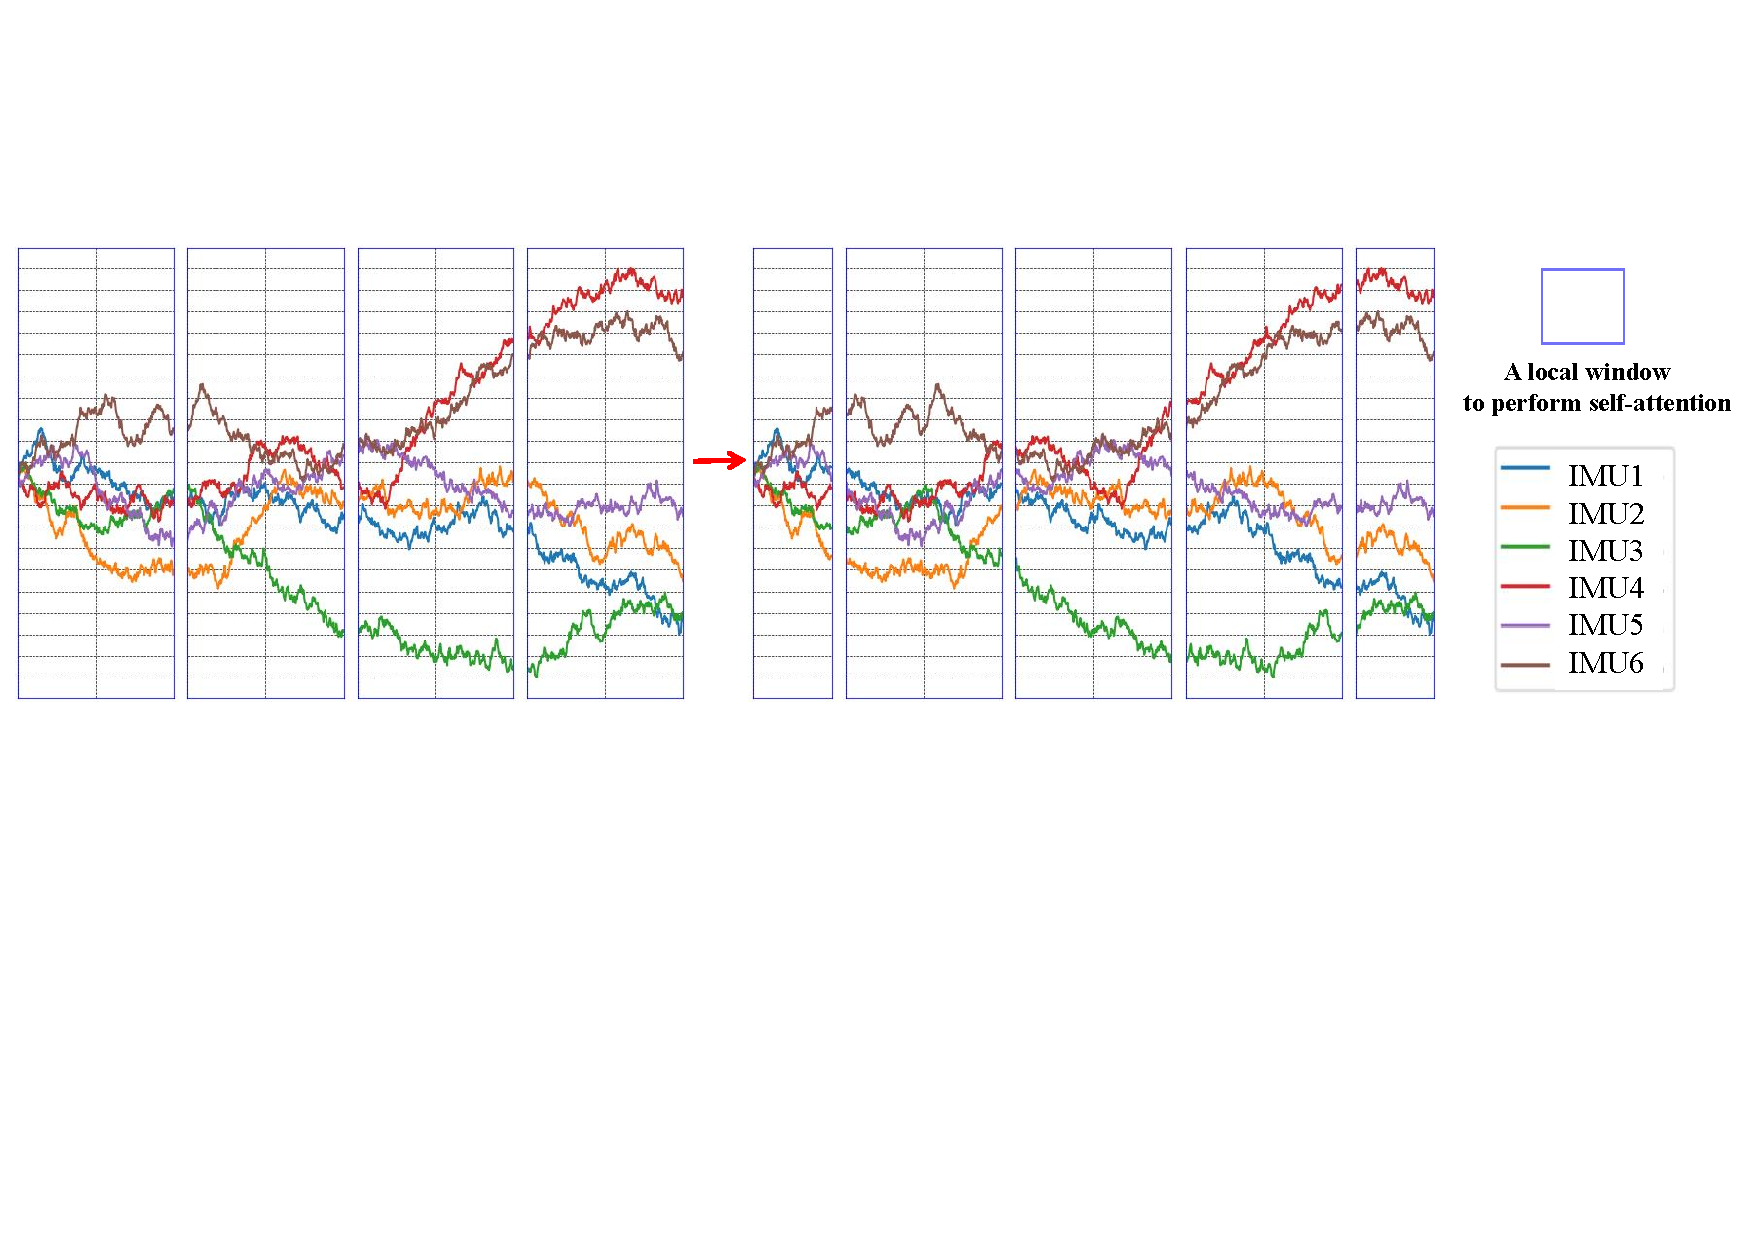
\includegraphics[width=\columnwidth]{window_partition.pdf} 
% An illustration of the W-SA and the SW-SA. On the left, We divide the sensor sequence into non-overlapping sub-segments based on a predefined window size. Computations for local window attention are then performed within these segments. In a quest to foster interrelations among non-overlapping segments, we introduce a sliding window operation. This operation facilitates a novel window partitioning scheme where the self-attention computation is carried out, as illustrated on the right.
% On the left, W-SA divides the sensor sequence into non-overlapping segments for localized attention. In a quest to foster interrelations among non-overlapping segments, SW-SA implements a sliding window technique, enabling a new partitioning method that enhances self-attention across segments as demonstrated on the right.
\caption{An illustration of window self-attention (left) and shifted window self-attention (right).}
\label{fig3}
\end{figure}





\subsection{Text-Sensor Fusion Module} 
%先去看一下后面的模型设计
The Text-Sensor Fusion Module aligns and fuses bimodal features.
Specifically, we employ a Hierarchical Temporal Transformer to acquire spatiotemporally fused sensor features for temporal synchronization with text features. Subsequently, contrastive learning is used to align the multimodal features in a high-dimensional space, followed by the application of cross-attention for feature fusion.
% The Text-Sensor Fusion Module is designed to bridge the temporal alignment and fusion between the spatial-relation features of IMUs and the textual semantics. We design a Hierarchical Temporal Transformer to obtain the temporal tokens from the spatial-relation features. In addition, contrastive learning and cross attention are employed to align and fuse the temporal tokens and the textual semantics.

\textbf{Hierarchical Temporal Transformer (HTT):} The HTT module is utilized for temporal alignment between sensor features and textual semantics. We hypothesized that information derived from adjacent frames is pivotal for the estimation of the current frame pose. In response to this hypothesis, window self-attention (W-SA) and shifted window self-attention (SW-SA) mechanisms are incorporated to constrain the scope of attention computation, introducing a convolution-like locality to the process.
Furthermore, to integrate information from distant frames and thus extend the receptive field, a patch merge operation is implemented. This approach facilitates the extraction of sensor features at diverse granularity levels and concurrently reduces the computational complexity of the transformer from a quadratic to a linear relationship with the sequence length.
% HTT module incorporates window self-attention (W-SA), shifted window self-attention (SW-SA), and a patch merging strategy. These components foster a linear relationship between computational complexity and input sequence length, enhancing the efficiency of temporal modeling.

Given a window size of $I$, a sensor sequence of length $L$ is divided into $\frac{L}{I}$ non-overlapping subintervals. Local window attention computations are first performed within these subintervals. To create interconnections between these non-overlapping segments, we adopt a shifted window attention module inspired by \cite{liu2021swin}, enabling a new partitioning method that enhances self-attention across segments. The W-SA and SW-SA always appear alternately, constituting a Hierarchical Transformer Block as shown in the top-right corner of Fig. \ref{fig2}.

% Upon completion of the attention computation, the original sequence order is reinstated via a window reversal operation.
% It's important to note that the local window attention and the shifted window attention always appear in alternating pairs. The associated computation methodology is as follows:
% \begin{align}
% & \hat{\mathbf{s}}^l=\mathrm{W}-\operatorname{SA}\left(\mathrm{LN}\left(\mathbf{s}^{l-1}\right)\right)+\mathbf{s}^{l-1}, \\
% & \mathbf{s}^l=\operatorname{MLP}\left(\mathrm{LN}\left(\hat{\mathbf{s}}^l\right)\right)+\hat{\mathbf{s}}^l, \\
% & \hat{\mathbf{s}}^{l+1}=\operatorname{SW-SA}\left(\mathrm{LN}\left(\mathbf{s}^l\right)\right)+\mathbf{s}^l, \\
% & \mathbf{s}^{l+1}=\operatorname{MLP}\left(\mathrm{LN}\left(\hat{\mathbf{s}}^{l+1}\right)\right)+\hat{\mathbf{s}}^{l+1},
% \end{align}

% In our implementation, $LN$ denotes LayerNorm, and $MLP$ refers to the Multilayer Perceptron. $ \hat{\mathbf{s}}^l$ and $\mathbf{s}^l$ symbolize the output features of the (shifted) window attention module and the MLP module for block $l$, respectively. During attention computations for W-SA and SW-SA, we also introduce relative positional encoding as per the approach outlined in \cite{liu2021swin}.

\begin{figure}[h]
\renewcommand{\baselinestretch}{1.0}
\centering 
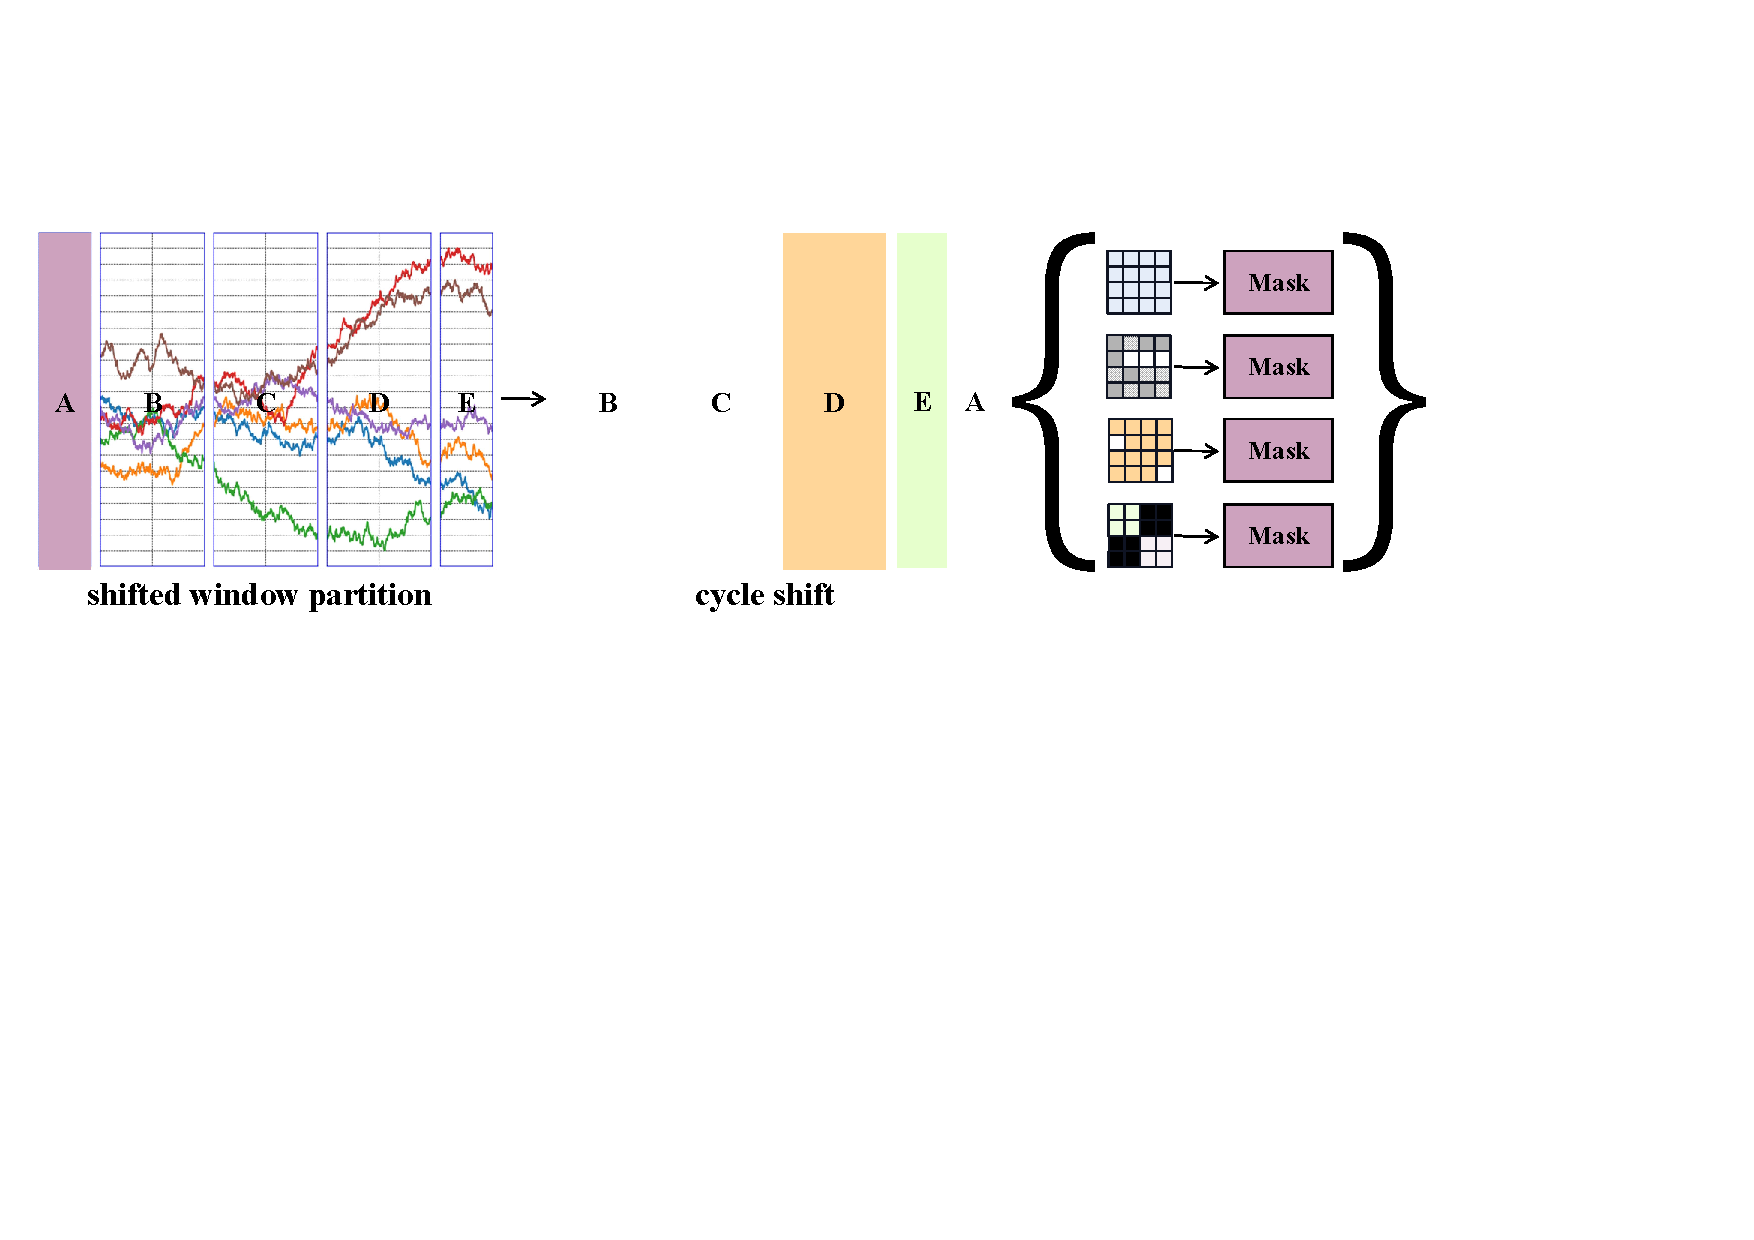
\includegraphics[width=0.92\columnwidth]{shift.pdf}
\caption{An efficient methodology for batch computation of self-attention within the context of shifted window partitioning.}\label{fig4}
\end{figure}
When applying shifted window attention to temporal sequences, the window count increases from $\frac{L}{I}$ to $\frac{L}{I} + 1$, resulting in some windows being smaller than $I$. To address this, we introduce a batch computation with a leftward cyclic shift, depicted in Fig. \ref{fig4}. This shift can produce windows with non-contiguous sub-windows. We tackle this by designing a masking mechanism that restricts self-attention to within each sub-window, maintaining the number of batched windows and ensuring computational efficiency. After the computation, the original sequence order is restored.
% In applying shifted window attention to temporal data, we encounter a challenge: the number of windows changes from $\frac{L}{I}$ to $\frac{L}{I}+1$, leading to some windows with a size less than $I$. To overcome this, we propose an enhanced batch computation approach, characterized by a leftward cyclic shift, as illustrated in Fig. \ref{fig7}. After the shift, a 
% window may encompass non-contiguous sub-window within the feature map. In response to this characteristic, we design a masking mechanism that confines the self-attention computation to each individual sub-window.
 % requiring a masking mechanism to restrict self-attention computation to each individual sub-window.
% This strategy ensures the number of batched windows aligns with the traditional window partitioning, preserving computational efficiency.

In the patch merge operation, each procedure consolidates two adjacent tokens into one, effectively halving the token count and doubling each token's dimensionality. These transformed tokens are then fed into the subsequent stages. Within the final stage, the patch merge is omitted, and tokens are restored to their original count and dimensions through linear projection and reshaping. 
Within a sensor sequence, we map the output features $F \in \mathbb{R}^{T\times C}$ to a feature with dimensions $1\times C$, serving as the [CLS] token. This [CLS] token, in conjunction with $F$, forms the cumulative output $\{F^{cls}, F^{1}, ..., F^{T}\}$, which encompasses the spatio-temporal features.

%基本照搬了swin的说法,后面可能需要改 这里还有两处未说,一个是attention mask的设置,另一个是cls token是如何处理的


%这里要详细叙述一下text encoder的性质,尤其是位置编码部分 组编码,怎么筛选的序列编码  reverse操作还没有说



% Given Motion feature $\{mcls, v^{1}, ..., v^{f} \}$ and Text feature $\{wcls, w^{1}, ..., w^{N}\}$ , we remove the CLS token and use them as inputs to the multimodal fusion module. In order to reduce computational cost, we also employ windowed attention. The motion sequence features are divided into non-overlapping sub-sequences according to window size$W$. When calculating cross-attention, each motion sub-sequence is used as a query, and the concatenation of the motion sub-sequence with the comprehensive semantic features of the entire motion sequence is used as key for the cross-attention computation.

% The output of the fusion encoder consists of rotational data $q_{t} \in R^{j\times6}$ for j key points, their corresponding three-dimensional positional information $p_{t} \in R^{j\times3}$, and the velocity data of the root node $v_{t} \in R^{3}$.
% we omit the [CLS] token and feed them into the Text-Sensor fusion module.

\textbf{Feature Fusion:}
Given the sensor features set $\{{F^{cls}, F^{1}, ..., F^{T}}\}$ and the text features set $\{{W^{cls}, W^{1}, ..., W^{N}}\}$, we apply contrastive learning to align these features in a high-dimensional joint space, utilizing the [CLS] tokens as anchors.
Subsequently, the sensor features are fused with textual features through cross-attention. Corresponding group embeddings and temporal position embeddings are designed for both textual and sensor features.
% To reduce computational demands, we partition the sensor sequence features into distinct sub-sequences for window attention like W-SA. During cross-attention computation, each sensor sub-sequence is used as a query, and its combination with the entire motion sequence serves as the key.
% Subsequently, the features from the sensor encoder, after self-attention computation, are fused with the textual features through cross-attention. Specially, for both the textual and motion features, we have designed corresponding group embeddings and temporal position embeddings\cite{vaswani2017attention} for each. 
% Moreover, to decrease computational demands, We partition the sensor sequence features into distinct sub-sequences to use window attention like W-SA on it. During the cross-attention computation, we use each sensor sub-sequence as a query. The combination of the sensor sub-sequence and the comprehensive semantic features of the entire motion sequence serves as the key.

% The output from the fusion encoder comprises rotational data $q_{t} \in R^{j\times6}$ for j key points, the corresponding three-dimensional position $p_{t} \in R^{j\times3}$, and the root node's velocity data $v_{t} \in R^{3}$.

\subsection{Losses} 
%这里少了不确定度的loss设计
We train our model with three objectives: uncertainty learning on the Sensor Encoder, Text-Sensor contrastive learning on the unimodal encoders and recon loss on the Text-Sensor Fusion module. 
The relevant equations are presented below. The parameters $\delta$, $\gamma$, $\lambda$, $\alpha$, $\beta$ are used to balance the different loss weights.

\textbf{Uncertainty Loss:} We aim to estimate the uncertainty of the input IMU data. Inspired by \cite{kendall2017uncertainties}, we set our uncertainty estimation loss as:
\begin{equation}
\mathcal{L}_\sigma = \frac{\delta}{T} \sum_{t=1}^T(\left\|\frac{({q}^t-\hat q^t)}{ \sum_{j=1}^6\sigma_j^{t}}\right\|^2 + \left\|\frac{({p}^t-\hat p^t)}{ \sum_{j=1}^6\sigma_j^{t}}\right\|^2 +\sum_{j=1}^6\left\|\sigma_j^{t}\right\|^2)
\end{equation}
The term $\sigma_j^{t}$ denotes the uncertainty of the $j$-th sensor at the $t$-th frame. The terms $||{q}^t -\hat q^t||^2$ and $||{p}^t - \hat p^t||^2$ represent the squared discrepancies between the predicted and true values of the joint rotation angles and the joint positions for the $t$-th frame, respectively.

\textbf{Contrastive Loss:} We use text-sensor contrastive learning to learn better unimodal representations before fusion. Given a batch of $B$ text-sensor pairs, the model learns to maximize the similarity between a sensor sequence and its corresponding text while minimizing the similarity with the other $B-1$ texts in the batch, and vice versa. 
% As illustrated by Equation \eqref{e4},\eqref{e5}.
\begin{align}
\mathcal{L}_{\text{contrastive}} = -\frac{\gamma}{2B} \sum_{i=1}^{B} \left(H1 + H2 \right)
\label{e4}
\end{align}
where
\begin{align}
H1 & = \log \frac{e^{s_{i, i} / \tau}}{\sum_{j=1}^{B}e^{s_{i, j} / \tau}}, \
H2 & = \log \frac{e^{s_{i, i} / \tau}}{\sum_{j=1}^{B}e^{s_{j, i} / \tau}}
\label{e5}
\end{align}

The $s_{i, j}$ represents the similarity calculated by cosine similarity between the $i$-th sensor sequence and the $j$-th text, and $\tau$ is a learnable temperature parameter that controls the concentration of the distribution.

\textbf{Recon Loss:} Our model is optimized to encapsulate motion characteristics by minimizing the $L_2$ losses on joint orientations $q$, joint locations $p$, and root speed $s$, as shown in Equations \eqref{e6} and \eqref{e7}.
\begin{equation}
\mathcal{L}_{\text{recon}} = \lambda \cdot {D}(q, \hat{q})+ \beta \cdot {D}(p, \hat{p}) + \alpha \cdot {D}(s, \hat{s}) 
\label{e6}
\end{equation}
where
\begin{equation}
{D}(x, \hat{x}) = \frac{1}{T}\sum_{t=1}^T\left|x^t-\hat{x}^t\right|^2
\label{e7}
\end{equation}
calculates the discrepancy between the model's predicted values $x^t$ and the true values $\hat{x}^t$ for the $t$-th frame.
 
The full objective of our model is:
 \begin{equation}
 \mathcal{L}=\mathcal{L}_\sigma+\mathcal{L}_{\text {contrastive}}+\mathcal{L}_{\text {recon}}
\end{equation}


% Additionally, to enhance the model's capacity to navigate the optimization landscape, we incorporate a dynamic learning rate adjustment strategy. Specifically, this strategy reduces the learning rate when the decrease in loss stagnates. 
%这里说一下那个学习率设置,窗口大小,滑动窗口大小
% \newcolumntype{Y}{>{\centering\arraybackslash}X} % 居中的 X 类型列
% \newcolumntype{Z}{>{\centering\arraybackslash}p{0.2in}} % 第一列特定宽度
% \begin{table*}[t]
% \centering
% \tiny
% \begin{tabularx}{\textwidth}{Z *{10}{Y}}  % Change c to X
% \hline
% \multirow{2}{*}{} & \multicolumn{5}{c}{DIP} & \multicolumn{5}{c}{Totalcapture} \\
% \cline{2-11}
%  & SIP Err(deg) & Ang Err(deg) & Pos Err(cm) & Mesh Err(cm) & Jitter $(10^{2}m/s^{3})$ & SIP Err (deg) & Ang Err(deg) & Pos Err(cm) & Mesh Err(cm) & Jitter  $(10^{2}m/s^{3})$ \\
% \hline
% Tip &16.89(+/-8.90)&9.18(+/-5.12)&  5.63(+/-3.45)&6.64(+/-3.99)&10.86(+/-6.89)&11.74(+/-6.75)&11.57(+/-5.12)&5.26(+/-3.00)&6.10(+/-3.44)&9.69(+/-6.68)\\
% Transpose* &17.13(+/-9.12)&8.93(+/-5.24)&6.06(+/-3.73)&7.19(+/-4.31)&6.24(+/-10.04)& 13.65(+/-7.83)& 11.84(+/-5.36)&5.64(+/-3.42)&6.35(+/-3.70)&8.05(+/-11.70)\\
% Transpose &14.36(+/-6.98)&7.68(+/-4.03)&5.03(+/-2.82)&5.97(+/-3.27)&1.22(+/-2.13)&12.30(+/-5.90)&11.34(+/-4.84)& 4.85(+/-2.63)&5.54(+/-2.89)&1.31(+/-2.43) \\
% % PIP &  &  &  &  &  &  &  &  &  &  \\
% ours &14.02(+/-6.83)&8.52(+/-4.64)&4.75(+/-2.67)&5.79(+/-3.19)&1.94(+/-1.79)&8.50(+/-4.59)&9.86(+/-4.29)&3.98(+/-2.16)&4.64(+/-2.45)&1.77(+/-1.58)\\
% ours*&14.74(+/-7.15)&8.50(+/-4.53)&4.87(+/-2.77)&5.85(+/-3.24)&6.62(+/-15.23)
% &9.33(+/-5.02)&10.35(+/-4.58)&4.26(+/-2.33)&4.91(+/-2.64)&6.30(+/-15.27)\\
% \hline
% \end{tabularx}
% \caption{Comparison of model performance on evaluation datasets, The * denotes the results obtained in online mode.}
% \label{your-label}
% \end{table*}
% \begin{table*}[t]
% \centering
% \tiny
% \begin{tabularx}{\textwidth}{*{11}{X}}  % Change c to X
% \hline
% \multirow{2}{*}{} & \multicolumn{5}{c}{DIP} & \multicolumn{5}{c}{Totalcapture} \\
% \cline{2-11}
%  & SIP Err(deg) & Ang Err(deg) & Pos Err(cm) & Mesh Err(cm) & Jitter $(10^{2}m/s^{3})$ & SIP Err (deg) & Ang Err(deg) & Pos Err(cm) & Mesh Err(cm) & Jitter  $(10^{2}m/s^{3})$ \\
% \hline
% W/O TEXT &14.67(+/-7.15)
% &8.38(+/-4.53)&4.78(+/-2.74)&5.74(+/-3.21)&2.90(+/-1.98)&8.91(+/-4.67)&10.17(+/-4.42)&4.09(+/-2.17)&4.72(+/-2.45)&2.65(+/-1.73)\\
% W/O UGSA &14.20(+/-7.03)&8.40(+/-4.55)&4.92(+/-2.78)&5.97(+/-3.31)&1.98(+/-1.87)&8.85(+/-4.79)&9.99 (+/-4.42)&4.09(+/-2.25)&4.74(+/-2.54)&1.72(+/-1.52)\\
% W/O HTT &14.02(+/-6.71)&8.75(+/-4.66)& 4.68(+/-2.61)&5.67(+/-3.13)&0.50(+/-1.22)&8.50(+/-4.69)&9.94(+/-4.42)&3.98 (+/-2.18)&4.64(+/-2.46)&0.38(+/- 1.11)\\
% \hline
% \end{tabularx}
% \caption{Comparison of ablation models}
% \label{your-label}
% \end{table*}

\section{Experiment}

% We describe the datasets, metrics and hyperparameter used for training and evaluation, and subsequently demonstrate the superior performance of our model in comparison to contemporary state-of-the-art methods.
% \begin{table}[h] 
% \renewcommand\baselinestretch{1.0}
% \renewcommand\arraystretch{1.0}
% \setlength{\abovecaptionskip}{2pt}
% \centering
% \caption{Offline comparison of model performance on evaluation datasets. Bold numbers indicate the best performing entries}\label{tab:model_complexity}
% \resizebox{\columnwidth}{!}{
%  \begin{tabular}{>{\centering\arraybackslash}m{3cm}|>{\centering\arraybackslash}m{4cm}|>{\centering\arraybackslash}m{4cm}} % 调整每列的宽度

% %\specialrule{0em}{0.8pt}{0.8pt}s
% \multicolumn{3}{c}{Transpose} \\ \hline
% Metric &DIP&Totalcapture  \\\hline
% SIP Err(deg) &13.97(+/-6.77)&12.30(+/-5.90)\\ \hline
% Ang Err(deg) &\textbf{7.62(+/-4.01)}&11.34(+/-4.84) \\ \hline
% Pos Err(cm) &4.90(+/-2.75)&4.85(+/-2.63) \\ \hline
% Mesh Err(cm) &5.83(+/-3.21)&5.54(+/-2.89)\\ \hline 
% Jitter ($10^{2}m/s^{3}$) &\textbf{1.19(+/-.76)}&\textbf{1.31(+/-2.43)} \\ \hline 
% \multicolumn{3}{c}{}\\
% \multicolumn{3}{c}{DIP} \\ \hline  % 合并的列在这里
% Metric &DIP&Totalcapture  \\\hline
% SIP Err(deg) &16.36(+/-8.60)&--\\ \hline
% Ang Err(deg) &14.41(+/-7.90)&-- \\ \hline
% Pos Err(cm) &6.98(+/-3.89)&-- \\ \hline
% Mesh Err(cm) &8.56(+/-4.65)&--\\ \hline 
% Jitter ($10^{2}m/s^{3}$) &23.87(+/-23.84)&--\\ \hline 
% \multicolumn{3}{c}{ }\\
% \multicolumn{3}{c}{Ours} \\ \hline  
% Metric &DIP&Totalcapture  \\\hline
% SIP Err(deg) &\textbf{13.34(+/-6.71)}&\textbf{7.92(+/-4.38)}\\ \hline
% Ang Err(deg) &8.33(+/-4.70)&\textbf{9.35(+/-4.10)}\\ \hline
% Pos Err(cm) &\textbf{4.71(+/-2.72)}&\textbf{3.70(+/-2.03)} \\ \hline
% Mesh Err(cm) &\textbf{5.75(+/-3.29)}&\textbf{ 4.32(+/-2.29)}\\ \hline 
% Jitter ($10^{2}m/s^{3}$) &1.81(+/- 1.72)&1.74(+/-1.55) \\ \hline 
% % 合并的列在这里
% \end{tabular}}
% \end{table}
% We outline the datasets and metrics employed for assessment, subsequently highlighting the superior performance of our model when juxtaposed with contemporary state-of-the-art methods.

\begin{table*}[ht]
	\fontsize{10}{12}\selectfont
	\resizebox{\linewidth}{!}{
	\begin{tabular}{c|ccccc|ccccc}
		\hline
		& \multicolumn{5}{c|}{Totalcapture} & \multicolumn{5}{c}{DIP-IMU} \\
		\cline{1-6} \cline{7-11}
		Method& SIP Err ($\rm{deg}$) & Ang Err ($\rm{deg}$) & Pos Err ($\rm{cm}$) & Mesh Err ($\rm{cm}$) & Jitter ($10^2\rm{m}/\rm{s}^3$) &
		SIP Err ($\rm{deg}$) & Ang Err ($\rm{deg}$) & Pos Err ($\rm{cm}$) & Mesh Err ($\rm{cm}$) & Jitter ($10^2\rm{m}/\rm{s}^3$) \\
		\hline
		
		SIP   & -- & -- &   -- & -- & -- & 
		       21.02 ($\pm$9.61) &  8.77 ($\pm$4.38) &  6.66 ($\pm$3.33) &  7.71 ($\pm$3.80) &  3.86 ($\pm$6.32) \\
		DIP  & -- & -- &   -- & -- & -- &
		       16.36 ($\pm$8.60) & 14.41 ($\pm$7.90) &  6.98 ($\pm$3.89) &  8.56 ($\pm$4.65) & 23.37 ($\pm$23.84) \\
		Transpose & 12.30($\pm$5.90) & 11.34 ($\pm$4.84) & 4.85 ($\pm$2.63) & 5.54 ($\pm$2.89) & \textbf{1.31 ($\pm$2.43)} &
		       13.97 ($\pm$6.77) & \textbf{7.62 ($\pm$4.01)} & 4.90 ($\pm$2.75) & 5.83 ($\pm$3.21) & \textbf{1.19 ($\pm$1.76)} \\ \hline
      Ours & \textbf{7.92 ($\pm$4.38)} & \textbf{9.35 ($\pm$4.10)} & \textbf{3.70 ($\pm$2.03)} & \textbf{4.32 ($\pm$2.29)} & 1.74 ($\pm$1.55) &
		       \textbf{13.34 ($\pm$6.71)} &  8.33 ($\pm$4.70) & \textbf{4.71 ($\pm$2.72)} & \textbf{5.75 ($\pm$3.29)} & 1.81 ($\pm$1.72) \\
		\bottomrule
	\end{tabular}}
 \caption{
	    In offline settings, our method is evaluated against SIP, DIP, and Transpose on the Totalcapture and DIP-IMU datasets, focusing on the assessment of body poses.
	    %
	    The mean values, along with the standard deviations (enclosed in parentheses), for the sip error, angular error, positional error, mesh error, and jitter error, are presented in the report. Bold numbers indicate the best performing entries.
	}
	\label{table1}
\end{table*}

\begin{table*}[ht]
	\fontsize{10}{12}\selectfont
	\resizebox{\linewidth}{!}{
	\begin{tabular}{c|ccccc|ccccc}
		\hline
		& \multicolumn{5}{c|}{Totalcapture} & \multicolumn{5}{c}{DIP-IMU} \\
		\cline{1-6} \cline{7-11}
		Method& SIP Err ($\rm{deg}$) & Ang Err ($\rm{deg}$) & Pos Err ($\rm{cm}$) & Mesh Err ($\rm{cm}$) & Jitter ($10^2\rm{m}/\rm{s}^3$) &
		SIP Err ($\rm{deg}$) & Ang Err ($\rm{deg}$) & Pos Err ($\rm{cm}$) & Mesh Err ($\rm{cm}$) & Jitter ($10^2\rm{m}/\rm{s}^3$) \\
		\hline
		DIP  & -- & -- & -- & -- & -- &
			   17.10 ($\pm$9.59) & 15.16 ($\pm$8.53) & 7.33 ($\pm$4.23) & 8.96 ($\pm$5.01) & 30.13 ($\pm$28.76) \\
    PIP  & -- & -- & -- & -- & -- &
			   15.02  &8.73 & 5.04 &5.95 & \textbf{2.4} \\
    TIP  & 11.74($\pm$6.75) &  11.57($\pm$5.12) &  5.26($\pm$3.00) & 6.10($\pm$3.44)& 9.69($\pm$6.68) &
			  15.33($\pm$8.44)  & 8.89($\pm$5.04) & 5.22($\pm$3.32) &6.28($\pm$3.89) & 10.84($\pm$6.87) \\
      Transpose& 13.65 ($\pm$7.83) &11.84 ($\pm$ 5.36) & 5.64 ($\pm$ 3.42) &6.35 ($\pm$ 3.70) & \textbf{8.05  ($\pm$11.70)}&  16.68 ($\pm$8.68) &8.85 ($\pm$ 4.82) &5.95 ($\pm$ 3.65) & 7.09 ($\pm$ 4.24) &6.11  ($\pm$7.92) \\ \hline
         	Ours & \textbf{9.67 ($\pm$5.12)} & \textbf{10.49 ($\pm$ 4.55)} & \textbf{4.36 ($\pm$ 2.37)} & \textbf{5.05 ($\pm$ 2.69)} & 13.30 ($\pm$16.86) &
		       \textbf{14.18 ($\pm$7.14)} & \textbf{8.25 ($\pm$ 4.45)} & \textbf{4.76 ($\pm$ 2.76)} & \textbf{5.80 ($\pm$ 3.26)} & 14.41  ($\pm$17.18) \\
		\bottomrule
	\end{tabular}}
 \caption{
	    In online settings, our method is evaluated against DIP, PIP, TIP, and Transpose on the Totalcapture and DIP-IMU datasets, focusing on the assessment of body poses. Bold numbers indicate the best performing entries.
	}
	\label{table2}
\end{table*}



\subsection{Dataset Setting}
% In our experiment, we utilized two types of data: human motion datasets containing IMU data, and text sequences containing semantic annotations corresponding to the motion sequences.
Our experiment employed two types of data: sensor data captured during human motion and the corresponding textual annotations.
% For the semantic information, we employed the Babel dataset\cite{BABEL:CVPR:2021}. Babel is a comprehensive dataset featuring language labels that elucidate the actions performed in motion reconstruction (mocap) sequences. It provides annotations for approximately 43 hours of mocap sequences from AMASS\cite{mahmood2019amass}. The labelling operates on two levels of abstraction: sequence labels, which outline the overall action in the sequence, and frame labels, which detail every action in each sequence frame. Each frame label is meticulously aligned with the duration of the corresponding action in the mocap sequence, enabling the overlap of multiple actions.It is worth noting that since Babel does not provide semantic annotations for the DIP dataset, we manually annotated the DIP dataset at a sequence level. However, these semantic details are less comprehensive than those provided by Babel.

We utilized the Babel dataset \cite{BABEL:CVPR:2021} for semantic annotations, which provides two levels of text labels for around 43 hours of AMASS mocap sequences \cite{mahmood2019amass}: sequence labels describe the overall actions, while frame labels detail each action per frame. For the DIP-IMU dataset \cite{huang2018deep}, which lacks Babel's semantic annotations, we manually added sequence-level labels, albeit less comprehensive.

% Regarding the motion data, the scarcity of real datasets, coupled with the extensive data demands intrinsic to the deep learning training process, led us to adhere to previous methodologies. As a result, we synthesized inertial data for the AMASS dataset, which is significantly larger and contains more variations.We utilized the synthesized dataset in conjunction with the real dataset for training. The detailed dataset configuration is as follows:
Regarding the motion data, given the scarcity of real datasets and the extensive data requirements inherent in deep learning, we followed previous method \cite{jiang2022transformer} and synthesized more diverse inertial data from the extensive AMASS dataset. This enriched synthesized data, combined with real data, was used for training. The configuration details of the motion datasets are as follows:

\textbf{AMASS:} The AMASS dataset unifies various motion reconstruction datasets. We synthesized a subset of AMASS, incorporating the CMU, Eyes Japan, KIT, ACCAD, DFaust 67, HumanEva, MPI Limits, MPI mosh, and SFU datasets.

\textbf{DIP-IMU:} The DIP-IMU dataset comprises IMU readings and pose parameters from approximately 90 minutes of activity by 10 subjects. We reserved Subjects 9 and 10 exclusively for evaluation and utilized the rest for training.

\textbf{Totalcapture:} The Totalcapture dataset \cite{trumble2017total} 
comprises 50 minutes of motion captured from 5 subjects. Following previous works, we used real IMU data for evaluation, but ground truth and synthesized IMU readings were still integrated into the training set. Due to missing semantic annotations from Babel in some sequences, only 27 fully annotated sequences were utilized.
% The Totalcapture dataset includes IMU readings, pose parameters, and global translations from about 50 minutes of motion by 5 subjects, each with 13 IMUs. We isolated real data for evaluation, yet incorporated its ground truth and synthesized IMU readings into the AMASS training set, as per previous works. Due to some Totalcapture motion sequences lacking semantic annotations from Babel, only sections with these annotations were used, specifically in 27 sequences.
%对于运动数据我们要强调一下toc的缩减以及其他运动数据集的设置
%对于语义信息我们要强调一下dip的问题
% \begin{table}[h] 
% \renewcommand\baselinestretch{1.0}
% \renewcommand\arraystretch{1.0}
% \setlength{\abovecaptionskip}{2pt}
% \centering
% \caption{Online Comparison of model performance on evaluation datasets. Bold numbers indicate the best performing entries}\label{tab:model_complexity}
% \resizebox{\columnwidth}{!}{
%  \begin{tabular}{>{\centering\arraybackslash}m{3cm}|>{\centering\arraybackslash}m{4cm}|>{\centering\arraybackslash}m{4cm}}

% %\specialrule{0em}{0.8pt}{0.8pt}s
% \multicolumn{3}{c}{Transpose} \\ \hline
% Metric &DIP&Totalcapture  \\\hline
% SIP Err(deg) &16.68(+/-8.68)&13.65(+/-7.83)\\ \hline
% Ang Err(deg) &8.85(+/-4.82)&11.84(+/-5.36) \\ \hline
% Pos Err(cm) &5.95(+/-3.65)&5.64(+/-3.42) \\ \hline
% Mesh Err(cm) &7.09(+/-4.24)&6.35(+/-3.70)\\ \hline 
% Jitter ($10^{2}m/s^{3}$) &\textbf{6.11(+/-7.92)}&\textbf{8.05(+/-11.70)} \\ \hline 
% \multicolumn{3}{c}{}\\
% \multicolumn{3}{c}{DIP} \\ \hline  % 合并的列在这里
% Metric &DIP&Totalcapture  \\\hline
% SIP Err(deg) &17.10(+/-19.59)&--\\ \hline
% Ang Err(deg) &15.16(+/-8.53)&-- \\ \hline
% Pos Err(cm) &7.33(+/-4.23)&-- \\ \hline
% Mesh Err(cm) &8.96(+/-5.01)&--\\ \hline 
% Jitter ($10^{2}m/s^{3}$) &30.13(+/-28.76)&--\\ \hline 
% \multicolumn{3}{c}{ }\\
% \multicolumn{3}{c}{TIP} \\ \hline  % 合并的列在这里
% Metric &DIP&Totalcapture  \\\hline
% SIP Err(deg) &15.33(+/-8.44)&11.74(+/-6.75)\\ \hline
% Ang Err(deg) &8.89(+/-5.04)&11.57(+/-5.12) \\ \hline
% Pos Err(cm) &5.22(+/-3.32)&5.26(+/-3.00) \\ \hline
% Mesh Err(cm) &6.28(+/-3.89)&6.10(+/-3.44)\\ \hline 
% Jitter ($10^{2}m/s^{3}$) &10.84(+/-6.87)&9.69(+/-6.68) \\ \hline 
% \multicolumn{3}{c}{ }\\
% \multicolumn{3}{c}{Ours} \\ \hline  
% Metric &DIP&Totalcapture  \\\hline
% SIP Err(deg) &\textbf{14.47(+/-7.20)}&\textbf{9.75(+/-5.34)}\\ \hline
% Ang Err(deg) &\textbf{8.25(+/-4.49)}&\textbf{10.51(+/-4.65)}\\ \hline
% Pos Err(cm) &\textbf{4.80(+/-2.82)}&\textbf{4.39(+/-2.42)} \\ \hline
% Mesh Err(cm) &\textbf{5.82(+/-3.33)}&\textbf{ 5.06(+/-2.74)}\\ \hline 
% Jitter ($10^{2}m/s^{3}$) &14.13(+/- 17.83)&12.62(+/-16.90) \\ \hline 
% % 合并的列在这里
% \end{tabular}}
% \end{table}
\subsection{Metric}

For a fair comparison, we adhered to the evaluation methodology previously used for \cite{yi2021transpose}. We used five metrics for pose evaluation: 1) SIP error, which measures the average global rotation error of the limbs in degrees; 2) Angular error, the average global rotation error of all body joints, also in degrees; 3) Positional error, the average Euclidean distance error of all joints, with the spine aligned, measured in centimeters; 4) Mesh error, the average Euclidean distance error of the body mesh vertices, with the spine aligned, also in centimeters; 5) Jitter error, the average jerk of all body joints in predicted motion, which reflects motion smoothness.



\subsection{Training Details}

The entire training and evaluation regimen was conducted on a system equipped with 1 Intel(R) Xeon(R) Silver 4110 CPU and 1 NVIDIA GeForce RTX 2080 Ti GPU. Our model was developed using PyTorch 1.13.0, further accelerated by CUDA 11.6. Our model configuration sets the input sequence length $T$ at 80 frames, with a window and shifted size of 20 and 10 frames, respectively, and a threshold of $M$ being 15. The training process, utilizing a batch size of 40, incorporates the Adam optimizer \cite{kingma2014adam} initialized with a learning rate of $2e^{-5}$. To balance the magnitude of the loss, we set $\lambda$ and  $\alpha$ to 1, $\beta$ to 10, $\delta$ to 0.1, and $\gamma$ to 0.01. We focus on regressing information for the 15 major joints as defined in the SMPL model, instead of all joints. Additionally, we apply a moving average with a window size of 15 to the model's output, enhancing the smoothness of the predicted poses.

\subsection{Comparisons}

Quantitative and qualitative comparisons with SIP \cite{von2017sparse}, DIP \cite{huang2018deep}, Transpose \cite{yi2021transpose}, PIP \cite{yi2022physical} and TIP \cite{jiang2022transformer} on the Totalcapture and DIP-IMU datasets. In this comparison, we utilized the best-performing models published by the authors. For TIP, the authors employed a human body format different from ours. Therefore, we converted TIP's output into our format before conducting the comparison. 
% Specifically, as stated earlier, we diverge from previous setups by exclusively using the portion of the Totalcapture dataset that contains semantic annotations for our tests.
\begin{figure}[h]
\centering
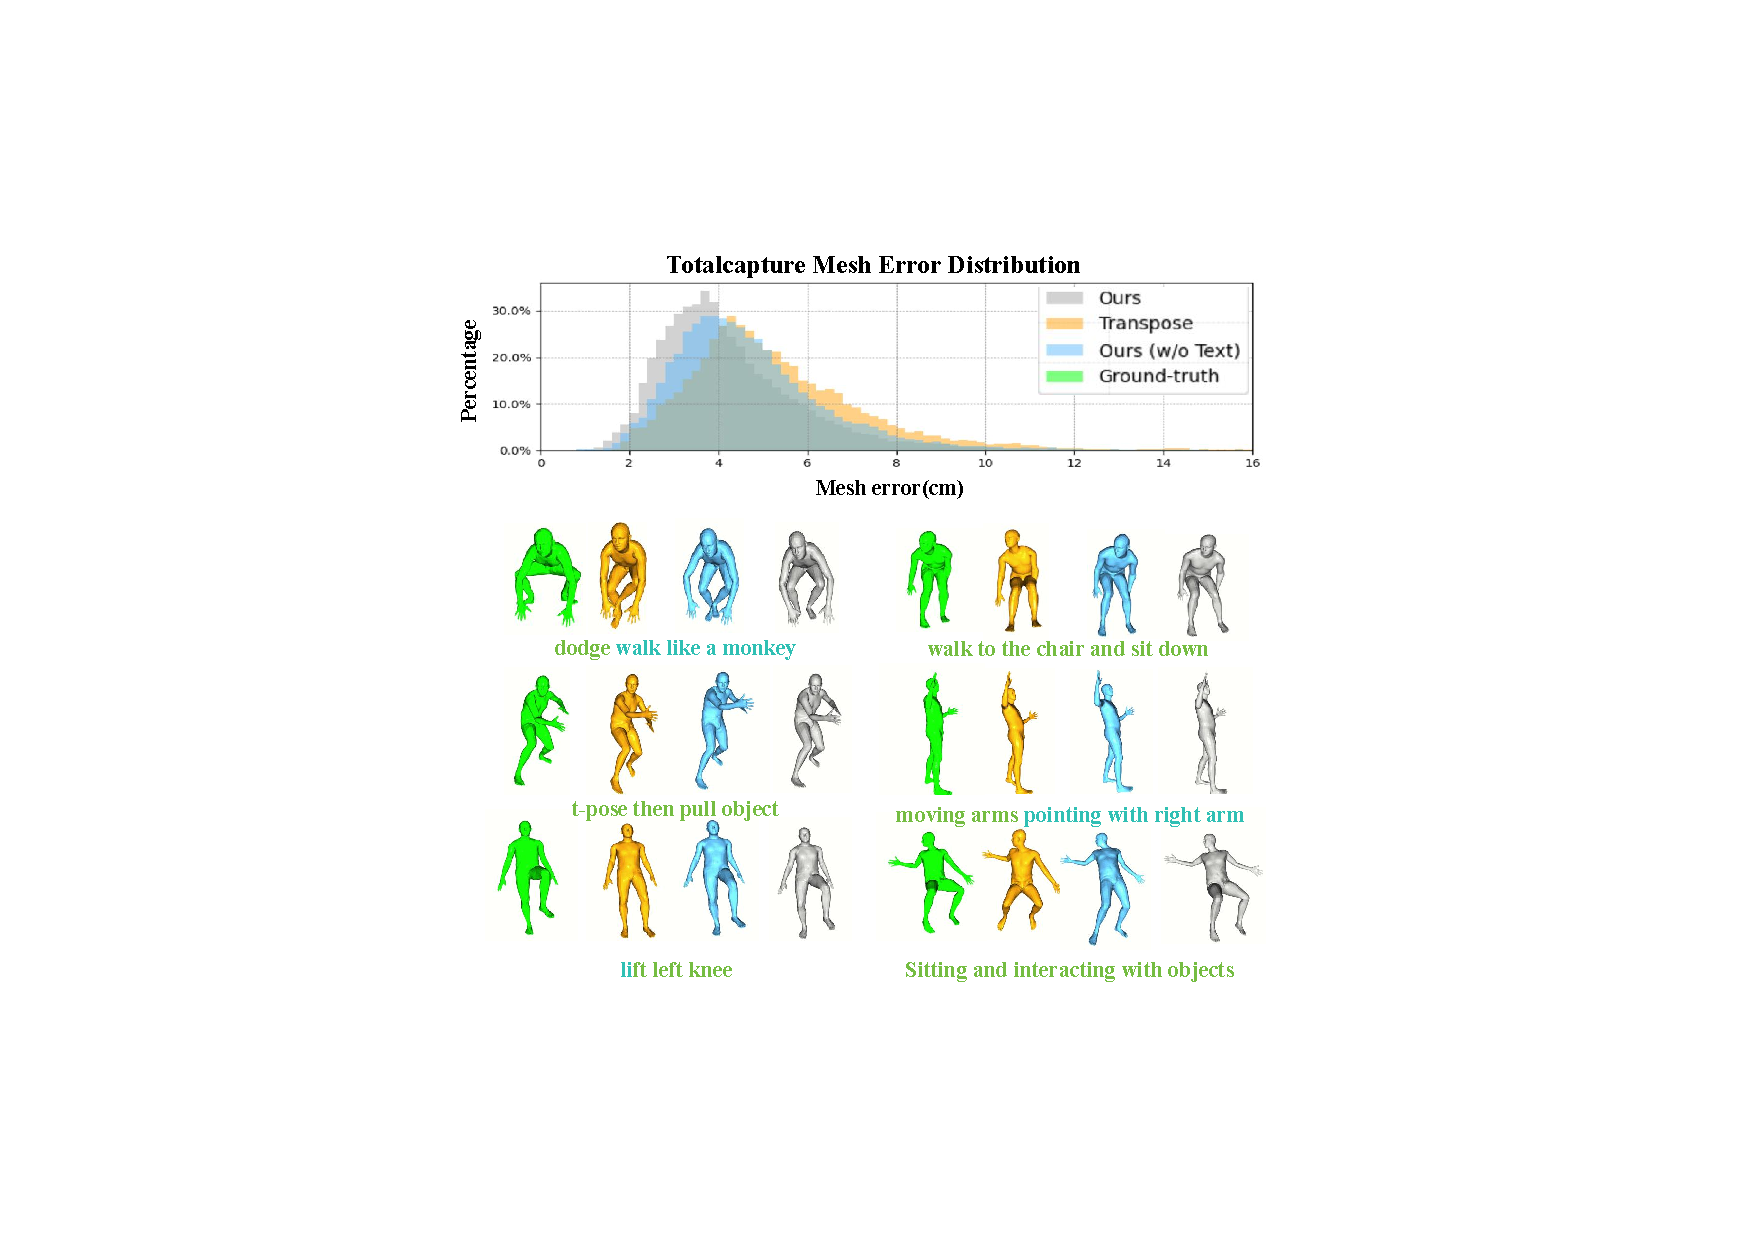
\includegraphics[width=\columnwidth]{Mesh_err.pdf} 
% Reduce the figure size so that it is slightly narrower than the column. Don't use precise values for figure width.This setup will avoid overfull boxes.
\caption{Mesh error distribution and qualitative comparisons between our method (with/without text) and Transpose. The text description of the motion is provided below, with the sequence label illustrated in green and the frame label presented in blue.}
\label{fig5}
\end{figure}
The results for the Totalcapture and DIP datasets setting in offline mode are presented in Table \ref{table1}.
Unlike previous methods, our approach does not consider all IMU readings when estimating the current pose. However, our method achieves satisfactory results after integrating semantic information. The performance of our method on the DIP dataset is not as impressive as on the Totalcapture dataset, which can be attributed to the DIP dataset's fewer and less detailed semantic annotations. 
% In Fig 4, we illustrate the comparison of the mesh error distribution and qualitative results between TransPose, which is currently the state-of-the-art (SOTA) method in offline mode, and our proposed method on the Totalcapture dataset. We have selected a few representative visual results to demonstrate the effectiveness of our method. 
As shown in Fig \ref{fig5}, our method excels in processing ambiguous actions like standing and sitting, and is adept at capturing finer details, such as the accurate alignment of hands and feet with the ground truth. This demonstrates a more natural, realistic, and precise performance.

% Our method excels at handling nuanced postures, as shown in Fig 6. Our motion closely aligns with the ground truth, demonstrating more natural, realistic, and precise performance.

It is worth noting that our full model cannot reconstruct human motion in real-time due to the requirement for semantic annotation. Therefore, we employ only the Sensor Encoder and the HTT module for the evaluation in real-time mode. Our method accesses 70 past frames, 5 current frames, and 5 future frames through a sliding window approach, with a tolerable latency of 83 ms. As shown in Table \ref{table2}, despite the absence of semantic information, our method still achieved superiority on multiple metrics, thereby validating the effectiveness of our network design.

The performance of our approach on the jitter metric is not as robust as other metrics, primarily owing to a constrained receptive field from the sliding window mechanism and the patch merging operation, which combines adjacent tokens into a single token. However, we posit that jitter,
unlike the other four pose-accuracy metrics, isn’t as critical. This perspective is based on the observation that visual discrepancies due to jitter are less noticeable when comparing our method with other approaches, while variations in pose precision are notably apparent.



\subsection{Ablation} 
We perform three ablations to validate our key design choices: (1) without text semantic information; (2) without the Uncertainty-guided Spatial Attention (UGSA) module; (3) without the Hierarchical Temporal Transformer (HTT) module. Table \ref{table3} summarizes the results on the Totalcapture dataset (offline).
Ablation experiments underscore the efficacy of our methodological design, with the integration of semantic information being the most salient contribution, followed by the implementation of UGSA and the HTT module.
% \begin{table}[h]
% \fontsize{10}{12}\selectfont
% \centering

% \renewcommand{\arraystretch}{1.7} % 调整行高的倍数
% \resizebox{\columnwidth}{!}{
%  \begin{tabular}{>{\centering\arraybackslash}m{2.5cm}|>{\centering\arraybackslash}m{2.5cm}|>{\centering\arraybackslash}m{2.5cm}|>{\centering\arraybackslash}m{2.5cm}|>{\centering\arraybackslash}m{2.5cm}}
%  \midrule
%  \multicolumn{5}{c}{Totalcapture}\\ % 在Totalcapture周围添加竖线和顶部水平线
%  \hline % 在Totalcapture下添加水平线
% Metric & w/o Text& w/o UGSA & w/o HTT & Ours \\\hline
% SIP Err(deg) &9.21(+/-4.75) &8.67(+/-4.73)  &  8.35(+/-4.57) &\textbf{7.92(+/-4.38)} \\ \hline
% Ang Err(deg) & 10.30(+/-4.43) & 9.94(+/-4.37) & 9.70(+/-4.29)&\textbf{9.35(+/-4.10)} \\ \hline
% Pos Err(cm) & 4.19(+/-2.23) & 4.04(+/-2.22) & 3.89(+/-2.10)&\textbf{3.70(+/-2.03)} \\ \hline
% Mesh Err(cm) &4.86(+/-2.54) &4.67(+/-2.50) &4.52(+/-2.35) &\textbf{ 4.32(+/-2.29)} \\ \hline
% Jitter ($10^{2}m/s^{3}$) & 1.87(+/-1.60) & 1.70(+/-1.55) &\textbf{0.44(+/-1.21)}&1.74(+/-1.55) \\ \hline


% \end{tabular}}
% \caption{Evaluation of Ablation Models on the  Totalcapture Dataset. Bold numbers indicate the best performing entries.}\label{table3}
% \end{table}

\begin{table}[h]
\fontsize{12}{14}\selectfont
\centering
\renewcommand{\arraystretch}{1.7} % Adjust the row height multiplier
\resizebox{\columnwidth}{!}{
 \begin{tabular}{
 >{\centering\arraybackslash}m{2.5cm}|>{\centering\arraybackslash}m{2.5cm}|>{\centering\arraybackslash}m{2.5cm}|>{\centering\arraybackslash}m{2.5cm}|>{\centering\arraybackslash}m{2.5cm}|>{\centering\arraybackslash}m{2.5cm}}
 % \midrule
% & \multicolumn{5}{c}{Totalcapture} \\ % Add vertical lines around Totalcapture and top horizontal line
 \hline % Add horizontal line under Totalcapture
 Method& SIP Err(deg) & Ang Err(deg) & Pos Err(cm) & Mesh Err(cm) & Jitter ($10^{2}m/s^{3}$) \\\hline
w/o Text & 9.21(+/-4.75) & 10.30(+/-4.43) & 4.19(+/-2.23) & 4.86(+/-2.54) & 1.87(+/-1.60) \\ 
w/o UGSA & 8.67(+/-4.73) & 9.94(+/-4.37) & 4.04(+/-2.22) & 4.67(+/-2.50) & 1.70(+/-1.55) \\ 
w/o HTT & 8.35(+/-4.57) & 9.70(+/-4.29) & 3.89(+/-2.10) & 4.52(+/-2.35) & \textbf{0.44(+/-1.21)} \\ \hline
Ours & \textbf{7.92(+/-4.38)} & \textbf{9.35(+/-4.10)} & \textbf{3.70(+/-2.03)} & \textbf{4.32(+/-2.29)} & 1.74(+/-1.55) \\ \hline
\end{tabular}}
\caption{Evaluation of Ablation Models on the Totalcapture Dataset. Bold numbers indicate the best performing entries.}\label{table3}
\end{table}

Without semantic information, the model's predictions fluctuate in ambiguous situations, a phenomenon illustrated in Fig. \ref{fig6} by the erratic alternation between sitting and standing positions. By incorporating a simple semantic annotation like ``sitting'', our model is able to maintain the desired sitting posture effectively.
% Fig \ref{fig5} shows a comparison between our method and the transpose technique, with and without semantic information. Without semantic information, the model's predictions fluctuate in ambiguous situations, as evidenced by the erratic alternation between sitting and standing positions. By incorporating a simple semantic annotation like 'sitting,' our model is able to maintain the desired sitting posture effectively.

% Fig \ref{fig5} presents a visual comparison between our method and the transpose technique, highlighting the differences with and without the incorporation of semantic information. As anticipated, the exclusion of semantic information from the model input resulted in fluctuating predictions for ambiguous situations - a challenge noted in previous studies. This issue led model to produce an erratic motion, continuously toggling between sitting and standing, instead of sustaining a stable sitting position. However, the incorporation of a simple semantic annotation, such as 'sitting', empowered our model to maintain the sitting posture effectively. 

Our findings indicate that the absence of Uncertainty-guided Spatial Attention affects the accuracy of the results. Fig. \ref{fig7} illustrates how uncertainty fluctuates over time. Uncertainty increases across all sensors during complex movements like squatting and crawling, particularly in the hand regions. Conversely, a transition to a standing posture leads to a marked reduction in uncertainty, with the leg sensors showing the lowest levels.

In examining the Hierarchical Temporal Transformer (HTT), we discern that employing window attention and patch merging within this module, instead of global attention, not only curtails computational needs but also elevates performance in almost all metrics, barring jitter. We consider such a trade-off to be acceptable.
% The lack of Uncertainty-guided spatial attention notably hindered the accuracy of the outcomes. Regarding the Hierarchical Temporal Transformer, we observe that utilizing window attention and patch merge within the HTT module, as opposed to global attention, not only diminishes computational requirements but also enhances performance across all measurements, with the exception of jitter. We regard this trade-off as judicious and well-founded. 

These ablation findings affirm our approach's superior capacity for modeling sensor information and its ability to leverage semantic cues for generating more precise and natural movements. 





\begin{figure}[t]
\centering
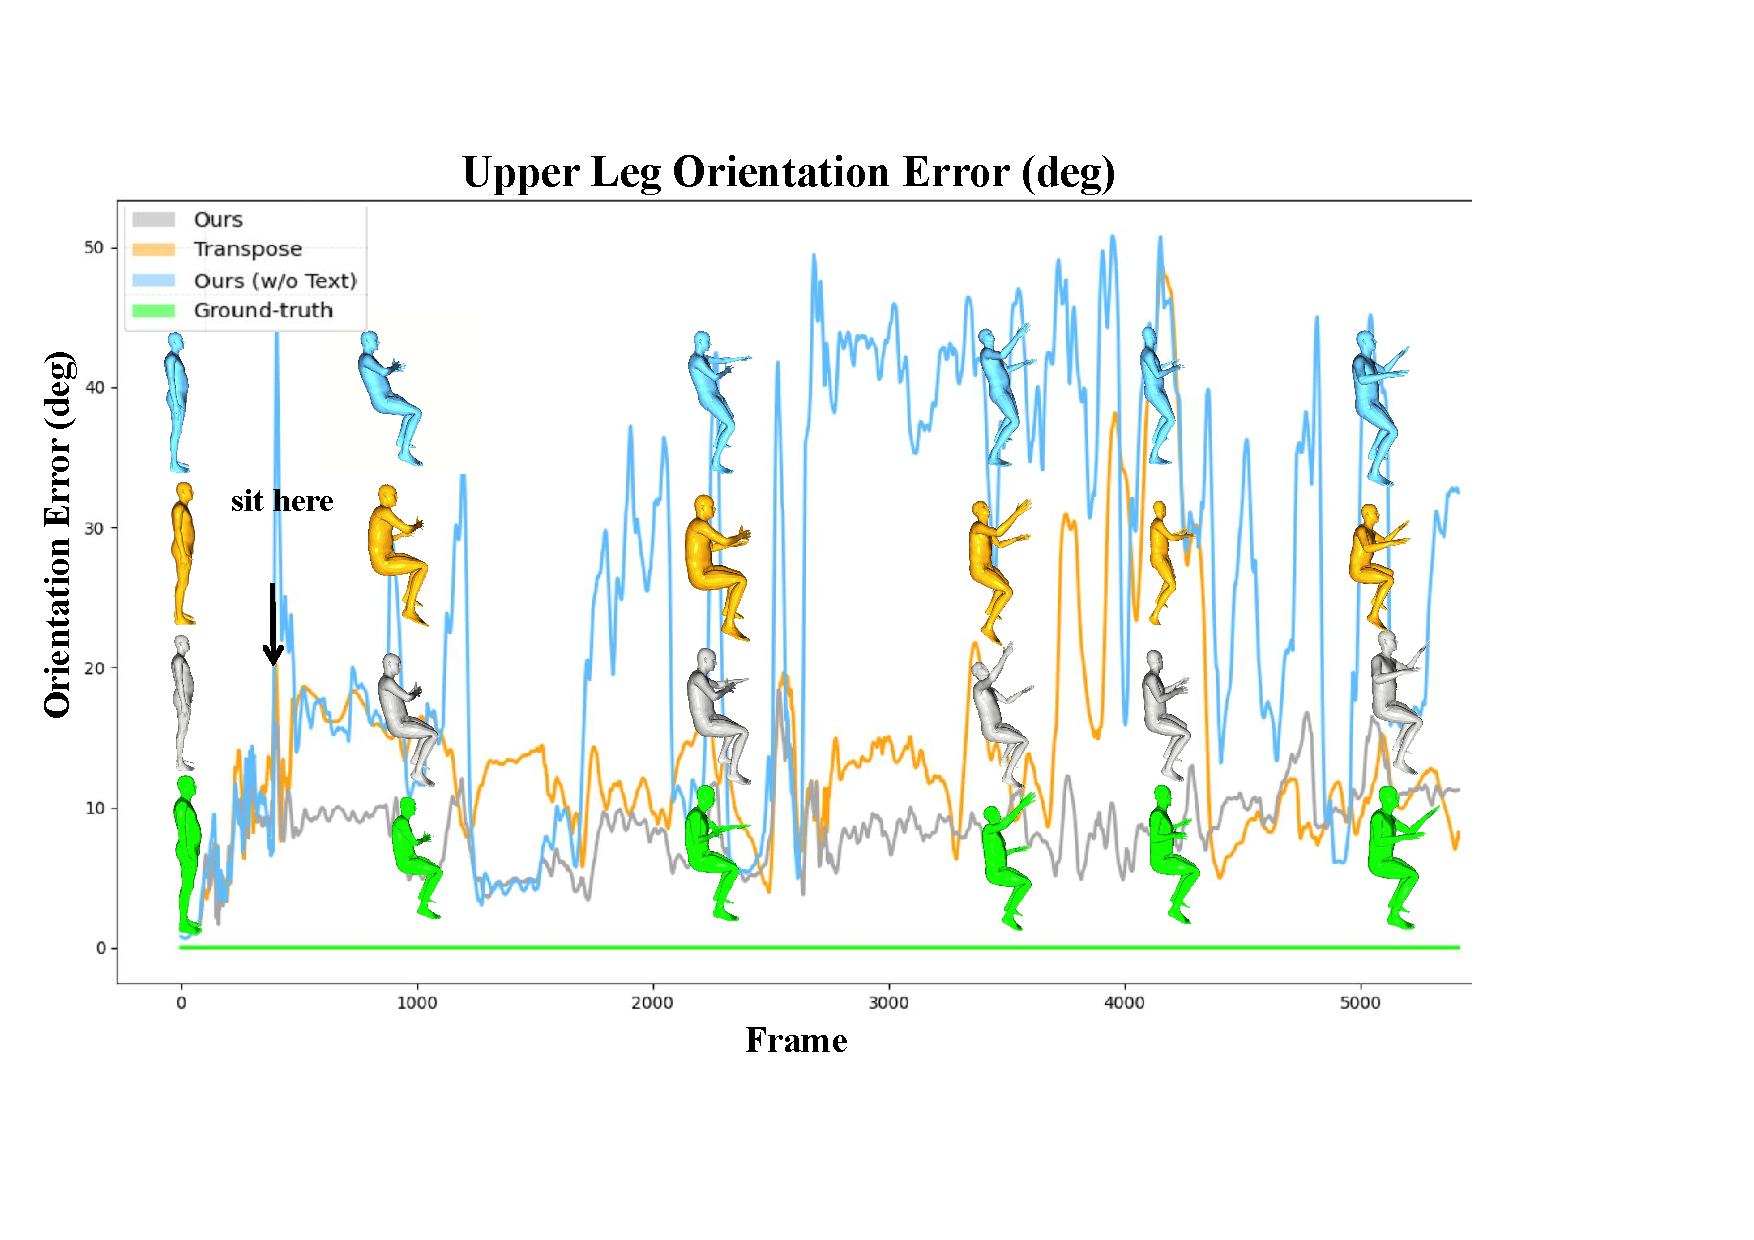
\includegraphics[width=\columnwidth]{sit.pdf} 
% Reduce the figure size so that it is slightly narrower than the column. Don't use precise values for figure width.This setup will avoid overfull boxes.(with or without text information)
\caption{We demonstrated a comparison between our method (with/without text) and Transpose in a sitting situation, focusing on the analysis of upper leg rotation error.}
\label{fig6}
\end{figure}
\begin{figure}[t]
\centering
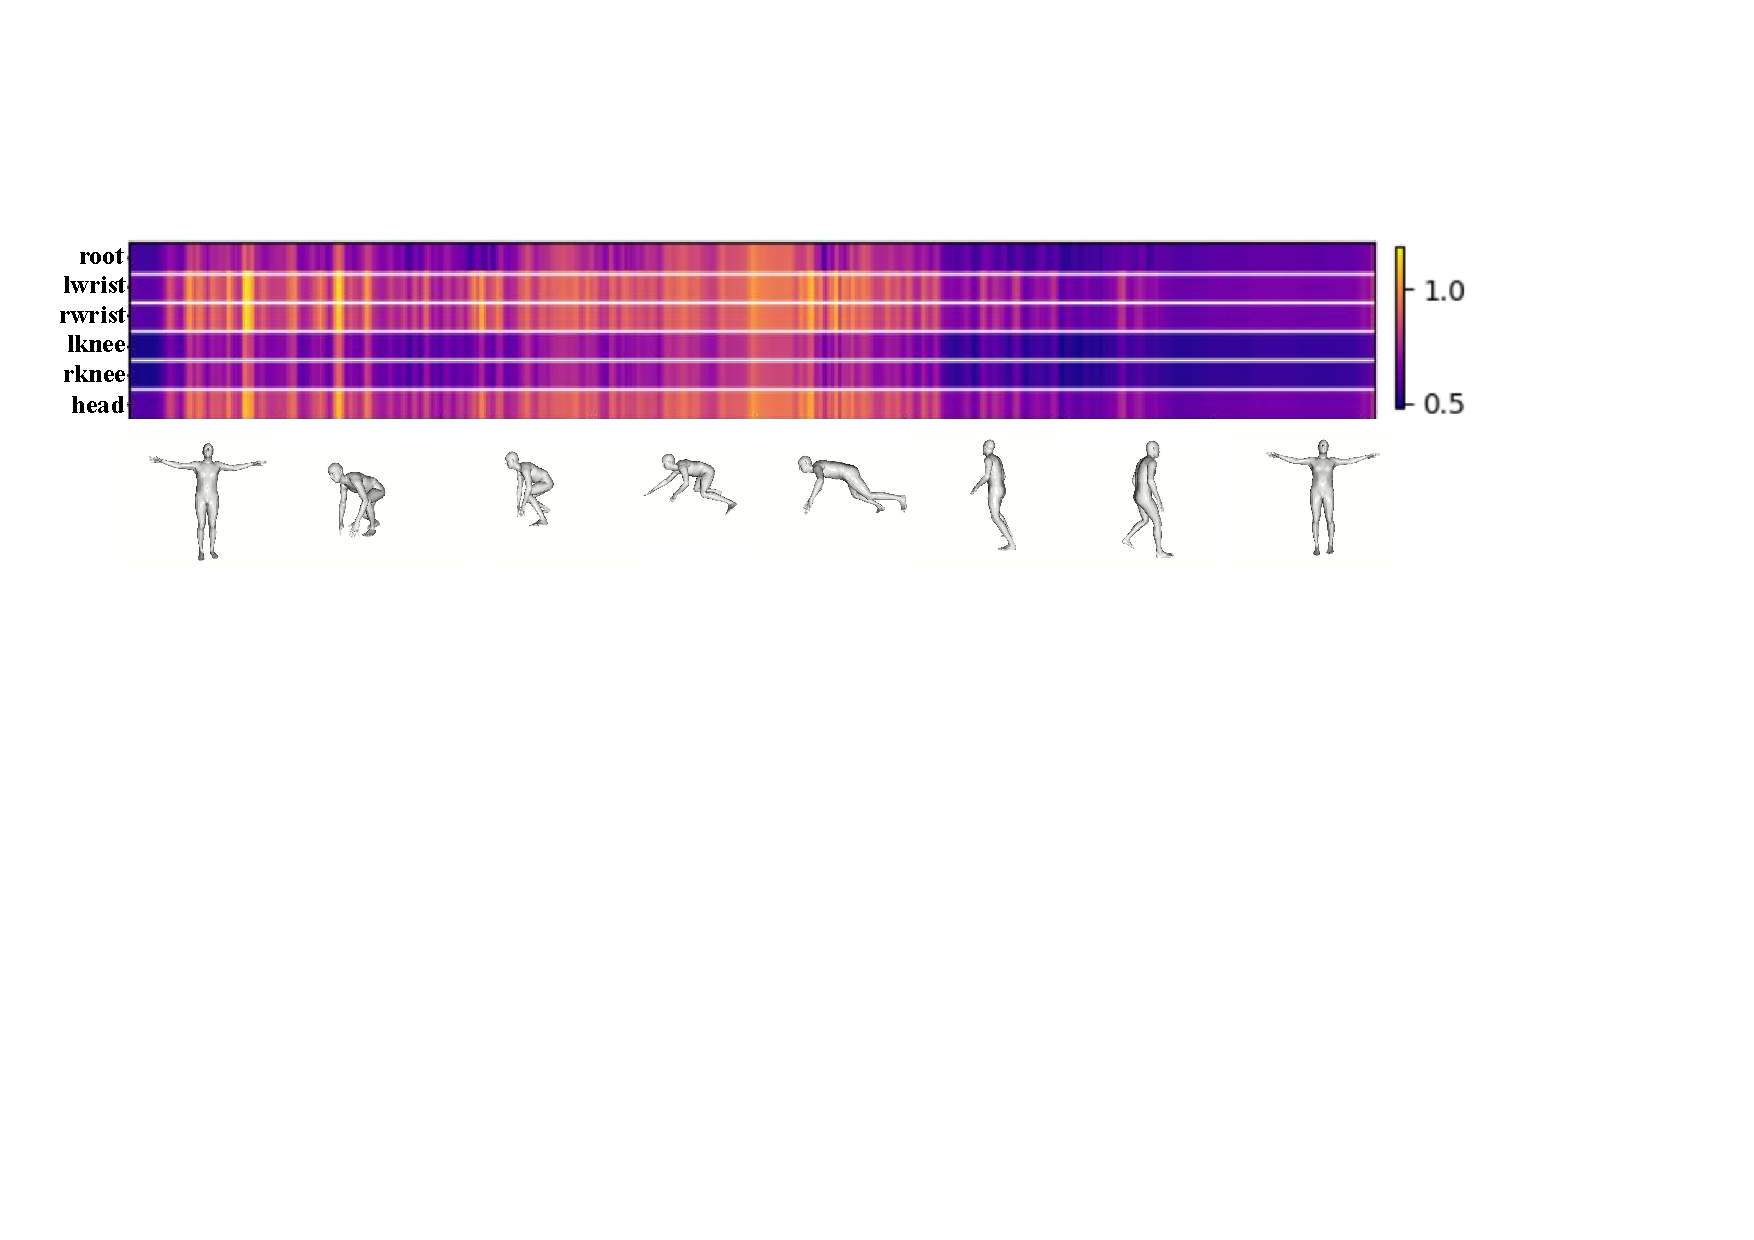
\includegraphics[ width=\columnwidth, keepaspectratio]{Uncertainty.pdf} 
% Reduce the figure size so that it is slightly narrower than the column. Don't use precise values for figure width.This setup will avoid overfull boxes.
\caption{Temporal Evolution of Uncertainty Across Six Sensors: Each row represents a different sensor, with color variations indicating changes in uncertainty.}
\label{fig7}
\end{figure}





\section{Conclusion}
In this paper, we are dedicated to addressing the ambiguity issues associated with using sparse inertial sensors for motion reconstruction.
Our approach involves enhancing the sensor data modeling capabilities and incorporating textual supervision. In the realm of sensor data modeling, we introduced an Uncertainty-guided Spatial Attention Module to model spatial relationships amongst IMUs while considering their respective uncertainty. For the modal fusion, we leverage the Hierarchical Temporal Transformer (HTT) module to achieve temporal alignment between sensor features and textual semantics. Furthermore, we employ contrastive learning to align features from both modalities in a high-dimensional space before fusion.
Experimental results have validated the effectiveness of our method. 
Looking ahead, we plan to explore the integration of real-time execution capabilities into our framework. This could include the combination of natural language reasoning with motion data, potentially utilizing ``prompt learning'' to train a decoder that performs real-time text annotation.
% The findings can be further applied to fields such as rehabilitation therapy assessment, action recognition research, and high-precision animation production.

\section{Acknowledgements}
This article is sponsored by National Key R\&D Program of China 2022ZD0118001, National Natural Science Foundation
of China under Grant 61972028, 62332017, 62303043 and U22A2022, and Guangdong Basic and Applied Basic Research Foundation
2023A1515030177, 2021A1515012285.

\bibliography{aaai24}



\end{document}
